\documentclass{scrartcl}

\usepackage{ucs}
\usepackage[utf8x]{inputenc}
\usepackage[ngerman]{babel}
\usepackage{graphicx}
\usepackage{amsmath}
\usepackage{amssymb}
\usepackage{color}
\usepackage{stmaryrd}

\title{Theoretische Informatik \\ Zusammenfassung}
\author{Thomas Mohr}
\date{}

\begin{document}
\maketitle
\pagebreak

\section{Alphabete, Worte, Sprachen}

\subsection{Alphabete und Worte}

\subsubsection{Definitionen und Beispiele}

\paragraph{Alphabete}

\begin{itemize}
	\item Ein Alphabet $\Sigma$ ist eine endliche Menge
	\item Die Elemente von $\Sigma$ nennt man \textbf{Zeichen} oder \textbf{Symbole}
	\item Für Alphabete benutzen wir große griechische Buchstaben $\mathbf{\Sigma,\Gamma,\ldots}$
	\item Für die Zeichen des Alphabets benutzen wir $\mathbf{a,b,c,\ldots}$
\end{itemize}

\paragraph{Worte}

\begin{itemize}
	\item Ein Wort über einem Alphabet $\Sigma$ ist eine endliche Folge von Zeichen aus $\Sigma$
	\begin{itemize}
		\item Beispiele
		\begin{itemize}
			\item Worte über $\{ 0,1 \}: \epsilon,0,1,01,1001,10101001, \ldots$
			\item Worte über $\{ a,\ldots,z \}: \epsilon,a,abra,anton,jkjhkjh,\ldots$
		\end{itemize}
	\end{itemize}
	\item Spezialfall: Das \textbf{leere Wort} = leere Folge von Zeichen = $\epsilon$
	\item $\Sigma^*$ := Menge aller Worte über dem Alphabet $\Sigma$
	\begin{itemize}
		\item Beispiele
		\begin{itemize}
			\item $\{ 1 \}^* = \{ \epsilon,1,11,111,1111,\ldots \}$
			\item $\{ 0,1 \}^* = \{ \epsilon,0,1,00,01,10,11,000,001,\ldots \}$
			\item $\{ a,\ldots,z \}^* = \{ \epsilon,a,b,\ldots,z,aa,ab,\ldots,ba,bb,bc,\ldots$
		\end{itemize}
	\end{itemize}
\end{itemize}

\paragraph{Wortdarstellung}

\begin{itemize}
	\item Es gibt zwei Methoden \textbf{nichtleere} Worte anzugeben
	\begin{enumerate}
		\item Durch Angabe der Folge aller Zeichen
		\begin{itemize}
			\item $abra,ojeoje,01001,7F3D,CAESAR,11111,\ldots$
		\end{itemize}
		\item Als $\mathbf{w = a.v}$, wobei
		\begin{itemize}
			\item $\mathbf{a}$ das erste Zeichen $(a \in \Sigma)$
			\item $\mathbf{v}$ das Restwort ist $(v \in \Sigma^*)$
		\end{itemize}
	\end{enumerate}
	\begin{itemize}
		\item Beispiel:
		\begin{itemize}
			\item $abra = a.bra = a.(b.ra) = a.(b.(r.a)) = a.(b.(r.(a.\epsilon)))$
		\end{itemize}
		\item Auf Klammern kann man verzichten
		\begin{itemize}
			\item $abra = a.bra = a.b.ra = a.b.r.a = a.b.r.a.\epsilon$
		\end{itemize}
	\end{itemize}
\end{itemize}

\subsubsection{Operationen mit Worten}

\begin{itemize}
	\item \textbf{Länge} (Anzahl der Zeichen)
	\begin{itemize}
		\item $|w|$ = Anzahl der Zeichen in $w$
		\item Formale Definition:
		\begin{enumerate}
			\item $|\epsilon| = 0 \hfill w = \epsilon$
			\item $|a.v| = 1 + |v| \hfill w = a.v$
		\end{enumerate}
	\end{itemize}
	\item \textbf{Konkatenieren} (Aneinanderhängen)
	\begin{itemize}
		\item $w = u \circ v = uv$
		\item Formale Definition:
		\begin{enumerate}
			\item $\epsilon \circ v = v \hfill u = \epsilon$
			\item $(a.u') \circ v = a.(u' \circ v) \hfill u = a.u'$
		\end{enumerate}
		 \item Wir identifizieren das Zeichen $a$ mit dem Wort $a.\epsilon$ (der Länge 1)
		 \item Für $\mathbf{a} \in \Sigma$ und $\mathbf{u} \in \Sigma^*$ also: $\mathbf{au}$ statt $\mathbf{(a.\epsilon) \circ u = a.u}$
	\end{itemize}
\end{itemize}

\paragraph{Reverse und Palindrome}

\begin{itemize}
	\item \textbf{Reverse}
	\begin{itemize}
		\item $w^R$ ist das \textbf{reverse Wort} zu $w$
		\item Formale Definition:
		\begin{enumerate}
			\item $\epsilon^R = \epsilon \hfill w = \epsilon$
			\item $(a.v)^R = v^R \circ (a.\epsilon) \hfill w = a.v$
		\end{enumerate}
	\end{itemize}
	\item \textbf{Palindrom}
	\begin{itemize}
		\item Wort $w$ mit $w^R = w$
		\item Formale Definition:
		\begin{enumerate}
			\item $\epsilon$ ist Palindrom
			\item Falls $u \neq \epsilon$
			\begin{enumerate}
				\item $a.\epsilon$ ist Palindrom
				\item $a.v$ ist Palindrom $\iff v = u \circ (a.\epsilon)$ und $u$ ist Palindrom
			\end{enumerate}
		\end{enumerate}
	\end{itemize}
\end{itemize}

\paragraph{Präfixe, Suffixe, Teilworte}

\begin{itemize}
	\item $\mathbf{u}$ ist \textbf{Präfix} von $w :\iff \exists v: \mathbf{u} \circ v = w$
	\begin{itemize}
		\item $\epsilon$ \textbf{Präfix} $w$
		\item $a.u$ \textbf{Präfix} $w \iff w= a.v \wedge u$ \textbf{Präfix} $v$
	\end{itemize}
	\item $\mathbf{v}$ ist \textbf{Suffix} von $w :\iff \exists u: u \circ \mathbf{v} = w$
	\begin{itemize}
		\item $u$ \textbf{Suffix} $w \iff u^R$ \textbf{Präfix} $w^R$
	\end{itemize}
	\item $\mathbf{t}$ ist \textbf{Teilwort} von $w :\iff \exists u,v: w = u \circ \mathbf{t} \circ v$
	\begin{itemize}
		\item $u$ \textbf{Teilwort} $w \iff u$ \textbf{Präfix} $w \vee w = a.v \wedge u$ \textbf{Teilwort} $v$
	\end{itemize}
\end{itemize}

\paragraph{Theoreme}

\begin{itemize}
	\item Es gelten u.a die Theoreme:
	\begin{enumerate}
		\item $\forall u,v,w \in \Sigma^*: (u \circ v) \circ w = u \circ (v \circ w)$
		\item $\forall u,v \in \Sigma^*: |u \circ v| = |u| + |v|$
		\item $\forall w \in \Sigma^*: |w^R| = |w|$
		\item $\forall u,v \in \Sigma^*: (u \circ v)^R = v^R \circ u^R$
	\end{enumerate}
\end{itemize}

\paragraph{Menge aller Worte über $\Sigma$}

\begin{itemize}
	\item $\Sigma^*$ ist \textbf{kleinste} Menge mit
	\begin{itemize}
		\item $\epsilon \in \Sigma^*$
		\item $\forall a \in \Sigma. \forall u \in \Sigma^*. a.u \in \Sigma^*$
	\end{itemize}
	\item Gleichheit
	\begin{align*}
		\forall u,v \in \Sigma^*: u = v \iff (u \equiv \epsilon \equiv v) \vee (u \equiv a.u' \wedge v \equiv a.v' \wedge u' = v')
	\end{align*}
\end{itemize}

\subsubsection{Induktionsbeweise}

\paragraph{Induktionsprinzip}

\begin{itemize}
	\item Sei $P: \Sigma^* \rightarrow \mathbb{B}$ eine ''\textbf{Wort-Eigenschaft}''
\end{itemize}

\begin{center}
	\renewcommand{\arraystretch}{1.25}
	\begin{tabular}[ht]{l c}
		$P(\epsilon)$ & Induktionsanfang \\ 
		$\forall a \in \Sigma. \forall v \in \Sigma^*. P(v) \implies P(a.v)$ & Induktionsschritt \\ 
		\hline 
		$\forall w \in \Sigma^*. P(w)$ & Induktionsschluss
	\end{tabular}
\end{center}

\paragraph{Ein Induktionsbeweis}

\begin{itemize}
	\item Behauptung: $\forall w \in \Sigma^*. w \circ \epsilon = w$
	\item Wähle: $P(w) := w \circ \epsilon = w$
	\begin{itemize}
		\item Induktionsanfang: $P(\epsilon)$
		\begin{align*}
			P(\epsilon) &\iff \epsilon \circ \epsilon \stackrel{\text{Def 1 } \circ}{=} \epsilon \\
			&\iff true
		\end{align*}
		\item Induktionsvoraussetzung: Für beliebige $a \in \Sigma, v \in \Sigma^*$ gelte $P(v)$
		\item Induktionsschritt: $\forall a \in \Sigma. \forall v \in \Sigma^*. P(v) \implies P(a.v)$
		\begin{align*}
			(a.v) \circ \epsilon & \stackrel{\text{Def 2 } \circ}{=} a.(v \circ \epsilon) \\
			& \stackrel{\text{IV}}{=} a.v
		\end{align*}
		\item Induktionsschluss: $\forall w \in \Sigma^*: P(w) \hfill \square$
	\end{itemize}
\end{itemize}

\subsection{Sprachen}

\subsubsection{Definitionen und Beispiele}

\paragraph{Formale Sprachen}

\begin{itemize}
	\item Eine Sprache \textbf{über einem Alphabet} $\mathbf{\Sigma}$ ist eine Menge von Worten aus $\Sigma^*$
	\item \textbf{Jede Teilmenge} $L \subseteq \Sigma^*$ ist eine Sprache
	\item Insbesondere auch:
	\begin{itemize}
		\item $\Sigma^* \hfill$ Menge aller Worte
		\item $\emptyset = \{\} \hfill$ leere Menge
		\item $\{ \epsilon \} \hfill$ Menge, die das leere Wort enthält
		\item $\{ a \}$ für $a \in \Sigma \hfill$ ein-elementige Menge mit Wort der Länge 1
	\end{itemize}
\end{itemize}

\paragraph{Beispiele formaler Sprachen}

\begin{itemize}
	\item Über dem Alphabet $\{ a,b,c \}$:
	\begin{itemize}
		\item $L_1 = \{ abba, cbc, a, \epsilon \} \hfill$ Sprache mit 4 Worten
		\item $L_2 = \{ a^nb^n \mid n \in \mathbb{N} \} \hfill$ beliebig viele $a$, dann gleich viele $b$
		\item $L_3 = \{ ucv \mid u,v \in \Sigma^* \} \hfill$ alle Worte, die ein c enthalten
	\end{itemize}
	\item über dem Alphabet $\{ 0,1,2,3,4,5,6,7,8,9 \}$:
	\begin{itemize}
		\item $L_4 = (\Sigma^* - \{ \epsilon \} - \{ 0w \mid w \in \Sigma^* \}) \cap \{ 0 \} \hfill \mathbb{N}$ in Dezimaldarstellung
	\end{itemize}
	\item über dem Alphabet $\{ (,) \}$:
	\begin{itemize}
		\item $L_5 =$ Menge aller ''\textbf{wohlgeformten}'' Klammerausdrücke (Dyck-Sprache)
		\begin{itemize}
			\item $(()(())) \in L_5$
			\item $(()))(() \not \in L_5$
		\end{itemize}
	\end{itemize}
\end{itemize}

\subsubsection{Operationen auf Sprachen}

\paragraph{''Reguläre'' Operationen auf Sprachen}

Seien $L, L_1, L_2 \subseteq \Sigma^*$ Sprachen.

\begin{itemize}
	\item $L_1 + L_2 := L_1 \cup L_2$
	\item $L_1 \circ L_2 := \{ u \circ v \mid u \in L_1, v \in L_2 \}$
	\item $L^n$ \textbf{rekursiv} definiert durch
	\begin{itemize}
		\item $L^0 := \{ \epsilon \}$
		\item $L^{n+1} := L \circ L^n$
	\end{itemize}
	\item $L^* := \bigcup_{n \leq 0} L^n$
\end{itemize}

\paragraph{Einige Gleichheiten}

\begin{itemize}
	\item $L,R,S$ seien beliebige Sprachen. Es gelten z.B.:
	\begin{itemize}
		\item $(L + R)S = LS +RS$
		\begin{itemize}
			\item Beweis:
			\begin{align*}
				w \in (L + R)S &\implies w = uv \text{ mit } (u \in L \text{ oder } u \in R) \text{ und } v \in S \\
				&\implies w = uv \in LS \text{ oder } w = uv \in RS
			\end{align*}
			\item Rückrichtung analog
		\end{itemize}
		\item $S(\bigcup_{n \in \mathbb{N}}R^n) = \bigcup_{n \in \mathbb{N}}(SR^n)$
		\begin{itemize}
			\item Beweis:
			\begin{align*}
				w \in S(\bigcup_{n \in \mathbb{N}}R^n) &\implies w = uv \text{ mit } u \in S \text{ und } v \in \bigcup_{n \in \mathbb{N}}R^n \\
				&\implies \exists n \in \mathbb{N}. v \in R^n \\
				& \implies \exists n \in \mathbb{N}. uv \in SR^n \\
				&\implies w = uv \in \bigcup_{n \in \mathbb{N}}SR^n
			\end{align*}
			\item Rückrichtung analog
		\end{itemize}
		\item $S(RS)^* = (SR)^*S$
		\begin{itemize}
			\item Beweis:
			\begin{align*}
				w \in S(RS)^* &\implies \exists n \in \mathbb{N}. \exists u_0, \ldots u_n \in S. \exists v_1, \ldots, v_n \in R. w = u_0(v_1u_1) \ldots (v_nu_n) \\
				&\implies w = (u_0v_1)(u_1v_2) \ldots (u_{n-1}v_n)u_n \\
				&\implies w \in (SR)^*S
			\end{align*}
		\end{itemize}
	\end{itemize}
\end{itemize}

\paragraph{Ausdrückbare Operationen}

\begin{itemize}
	\item Die folgenden Operationen sind mit Hilfe der regulären Operatoren ausdrückbar.
	\begin{itemize}
		\item $L^+ := LL^*$
		\item $L? := L + \{ \epsilon \}$
	\end{itemize}
	\item Alle \textbf{regulären Operatoren} sind \textbf{monoton}, d.h.
	\begin{align*}
		L_1 \subseteq M_1 \text{ und } L_2 \subseteq M_2 &\implies L_1 + L_2 \subseteq M_1 + M_2 \\
		&\implies L_1 \circ L_2 \subseteq M_1 \circ M_2
	\end{align*}
	\begin{align*}
		L \subseteq M \implies L^* \subseteq M^*
	\end{align*}
\end{itemize}

\paragraph{Weitere Operationen auf Sprachen}

\begin{itemize}
	\item $L, L_1, L_2 \subseteq \Sigma^*$ Sprachen und $e \in \Sigma$
	\begin{itemize}
		\item $L_1 \cap L_2 \hfill$ Schnitt
		\item $\Sigma^* - L \hfill$ Komplement
		\item $L^R := \{ w^R \mid w \in L \} \hfill$ Revers
		\item $L_e := \{ v \in \Sigma^* \mid e.v \in L \} \hfill$ Ableitung nach $e$
	\end{itemize}
	\item Diese Operationen sind \textbf{nicht} mit Hilfe der regulären Operatoren ausdrückbar
	\begin{itemize}
		\item Beweis für Komplement: $L_1 \subset L_2 \implies \Sigma^* - L1 \not \subset \Sigma^* - L2$
	\end{itemize}
\end{itemize}

\subsection{Spracherkennung}

\subsubsection{Entscheidbarkeit}

\begin{itemize}
	\item Eine Sprache $\mathbf{L \subseteq \Sigma^*}$ heißt \textbf{entscheidbar}, wenn es einen ''Algorithmus'' $E_L$ gibt, der zu jedem Input $\mathbf{w \in \Sigma^*}$ entscheidet, ob $\mathbf{w \in L}$ oder $\mathbf{w \in \Sigma^* - L}$
	\begin{itemize}
		\item $w \in L \iff E_L(w) = true$
		\item $w \not \in L \iff E_L(w) = false$
	\end{itemize}
	\item $E_L$ berechnet i.W. die \textbf{charakteristische Funktion} von $L$:
	\begin{align*}
		\chi_L(w) = \begin{cases}
			1 & \text{, falls } w \in L \\
			0 & \text{, falls } w \not \in L
		\end{cases}
	\end{align*}
\end{itemize}

\subsubsection{Semientscheidbarkeit}

\begin{itemize}
	\item Eine Sprache $L \subseteq \Sigma^*$ heißt \textbf{semi-entscheidbar}, wenn es einen ''Algorithmus'' $S_L$ gibt, der zu jedem Input $\mathbf{w \in \Sigma^*}$ bestätigen kann, falls $\mathbf{w \in L}$ ist
	\begin{itemize}
		\item $w \in L \iff S_L(w)$
		\item $w \not \in L \iff S_L(w) = false \vee S_L(w) = \bot$
	\end{itemize}
\end{itemize}

\paragraph{Entscheidbarkeit - Semi-Entscheidbarkeit}

\begin{itemize}
 	\item Eine Sprache $L \subseteq \Sigma^*$ ist \textbf{entscheidbar} $\iff L$ und $\Sigma^* - L$ sind semi-entscheidbar
 	\item Ist $L \subseteq \Sigma^*$ entscheidbar, so ist $L$ auch semi-entscheidbar
 	\begin{itemize}
 		\item Klar: $E_L(w) \implies S_L(w)$
 	\end{itemize}
 	\item Ist $L$ entscheidbar, dann ist das Komplement $\Sigma^* - L$ semi-entscheidbar
 	\begin{itemize}
 		\item Klar: $S_{\Sigma^* - L}(w) := \neg (E_L(w))$
	 \end{itemize}
 	\item Sind sowohl $L$ als auch $\Sigma^* - L$ semi-entscheidbar, dann ist $L$ entscheidbar:
 	\begin{itemize}
 		\item Lasse $S_L(w)$ und $S_{\Sigma^* - L}(w)$ parallel laufen
 		\item Falls $w \in L$ hält $S_L(w)$ mit $S_L(w) = true$
 		\item Falls $w \not \in S_{\Sigma^* - L}(w)$ hält $S_L(w)$ mit $S_{\Sigma^* - L}(w) = true$
 		\begin{align*}
			E_L(w) = \begin{cases}
				true & \text{, falls } S_L(w) = true \\
				false & \text{, falls } S_{\Sigma^* - L} = true
			\end{cases}
		\end{align*}
 	\end{itemize}
\end{itemize}

\pagebreak
\section{Reguläre Sprachen und reguläre Ausdrücke}

\begin{itemize}
	\item Sei $\Sigma$ ein Alphabet. \textbf{Reguläre Sprachen über} $\mathbf{\Sigma}$ sind induktiv definiert.
	\begin{enumerate}
		\item Regulär sind:
		\begin{itemize}
			\item $\emptyset \hfill$ die leere Sprache
			\item $\{ \epsilon \} \hfill$ enthält nur das leere Wort
			\item $\{ a \} \hfill \forall a \in \Sigma$
		\end{itemize}
		\item Abschlusseigenschaften
		\begin{itemize}
			\item Seien $L, L_1$ und $L_2$ reguläre Sprachen über dem Alphabet $\Sigma$, dann auch
			\begin{itemize}
				\item $L_1 \cup L_2 \hfill$ Vereinigung
				\item $L_1 \cap L_2 \hfill$ Schnitt
				\item $\Sigma^* - L = \overline{L} \hfill$ Komplement
				\item $\{ uv \mid u \in L_1 \wedge v \in L_2 \} \hfill$ Konketanation
				\item $L^* \hfill$ Kleene-Stern
				\item $L_1 \backslash L_2 \hfill$ Differenz
			\end{itemize}
		\end{itemize}
	\end{enumerate}
	\item Sei $\Sigma = \{ a_1, a_2, \ldots, a_n \}$ ein Alphabet. Dann sind die folgenden Sprachen regulär:
	\begin{itemize}
		\item $\Sigma \hfill$ denn $\Sigma = \{ a_1 \} \cup \{ a_2 \} \cup \ldots \cup \{ a_n \}$
		\item $\Sigma^* \hfill$ denn $\Sigma^* = \bigcup_{n \leq 0} \Sigma^n$
		\item $\{ w \}$ für jedes $w \in \Sigma^*$
		\begin{itemize}
			\item denn für $w = w_1w_2 \ldots w_n$ gilt $\{ w \} = \{ w_1 \} \{ w_2 \} \ldots \{ w_n \}$
			\item Jede \textbf{endliche Teilmenge} $L \subseteq \Sigma^*$
		\end{itemize}
		\item Ist $L$ regulär, dann auch
		\begin{itemize}
			\item $L^n = LL \ldots L \hfill$ n-mal für jedes $n \geq 0$
			\item $L^+ = LL^*$
			\item $L? = L \cup \{ \epsilon \}$
			\item $L^{\{  m,n \}} = L^m(\{ \epsilon \} \cup L \cup L^2 \cup \ldots \cup L^{n-m})$
			\item $L^{\{ m,^* \}} = L^mL^*$
		\end{itemize}
	\end{itemize}
\end{itemize}

\paragraph{Beispiele}

\begin{itemize}
	\item Reguläre Sprachen sind z.B.:
	\begin{itemize}
		\item $\{ a,b,abba, \epsilon \}$
		\item $\{ ba^nb \mid n \in \mathbb{N} \}$
		\item $\{ a^nba \mid n \text{ gerade} \}$
		\item $\{ a^nb^m \mid n,m \in \mathbb{N}, n \neq m \}$
		\item $\{ a^nb^m \mid n+m \text{ gerade} \}$
	\end{itemize}
	\item Keine regulären Sprachen sind
	\begin{itemize}
		\item $\{ a^nba^n \mid n \in \mathbb{N} \}$
		\item $\{ a^nb^m \mid n \leq m \}$
	\end{itemize}
\end{itemize}

\subsection{Syntaxdiagramme}

\begin{figure}[ht]
	\centering
	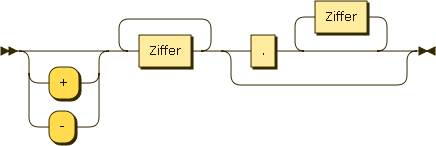
\includegraphics[scale=.5]{figures/Real.png}
	\caption{Real}
	\label{real}
\end{figure}

\begin{figure}[ht]
	\centering
	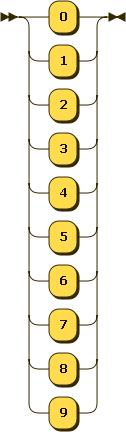
\includegraphics[scale=.5]{figures/Ziffer.png}
	\caption{Ziffer}
	\label{ziffer}
\end{figure}

\subsection{Ausdrücke über $\Sigma$}

\begin{itemize}
	\item Konstante Ausdrücke
	\begin{itemize}
		\item $\emptyset$
		\item $\epsilon$
		\item $a \hfill$ für jedes $a \in \Sigma$
	\end{itemize}
	\item Sind $e$ und $f$ reguläre Ausdrücke, dann auch
	\begin{itemize}
		\item $e + f$
		\item $ef$
		\item $e^*$
	\end{itemize}
	\item Ist $e$ regulärer Ausdruck, dann auch
	\begin{itemize}
		\item $(e)$
	\end{itemize}
\end{itemize}

\subsection{Semantik regulärer Ausdrücke}

\begin{itemize}
	\item Zu jedem regulären Ausdruck $e$ definiere eine Sprache $L(e)$:
	\begin{itemize}
		\item $L(\emptyset) := \{\}$
		\item $L(\epsilon) := \{ \epsilon \}$
		\item $L(a) := \{ a \}$ für jedes $a \in \Sigma$
	\end{itemize}
	\item und induktiv:
	\begin{itemize}
		\item $L(e + f) := L(e) \cup L(f)$
		\item $L(ef) := L(e) \circ L(f)$
		\item $L(e^*) := L(e)^*$
	\end{itemize}
	\item Beispiele:
	\begin{align*}
		L((0+1)^* 0 (1 + (01)^*)) &= (\{ 0 \} \cup \{ 1 \})^* \{ 0 \} (\{ 1 \} \cup \{ 01 \}^*) \\
		&= \{ 0,1 \}^* (\{ 01 \} \cup \{ 0 \}  \{ 01 \}^*) \\
		&= \{ 0,1 \}^* (\{ 01 \} \cup \{ 0 \}) \\
		&= \text{alle Worte, die auf 0 oder auf 01 enden}
	\end{align*}
	\begin{align*}
		L(e + \emptyset) &= L(e) \cup L(\emptyset) \\
		&= L(e) \cup \{\} \\
		&= L(e)
	\end{align*}
	\begin{align*}
		L(e \emptyset) &= L(e) \circ L(\emptyset) \\
		&= L(e) L(\emptyset) \\
		&= L(e) \{\} \\
		&= \{\}
	\end{align*}
	\begin{align*}
		L(e \epsilon) &= L(e) \{ \epsilon \} \\
		&= L(e)
	\end{align*}
\end{itemize}

\paragraph{Gleichungen}

\begin{itemize}
	\item \textit{Definition}: $r_1 \equiv r_2 :\iff L(r_1) = L(r_2)$
	\item Es gelten u.a.
	\begin{itemize}
		\item $\emptyset + e \equiv e$
		\item $e + f \equiv f + e$
		\item $(e + f) + g \equiv e + (f + g)$
		\item $\epsilon e \equiv e \equiv e \epsilon$
		\item $(ef) g \equiv e (fg)$
		\item $e(f + g) \equiv ef + eg$
		\item $(e + f)g \equiv eg + fg$
		\item $\epsilon^* \equiv \epsilon$
		\item $(e^*)^* \equiv e^*$
		\item $(\epsilon + e)^* \equiv e^*$
		\item $(e^*f^*)^* \equiv (e + f)^*$
		\item $(ef)^*e \equiv e(fe)^*$
	\end{itemize}
\end{itemize}

\paragraph{Herleitung}

\begin{align*}
	(ef + e)^* e &\equiv (ef + e \epsilon)^* e \\
	&\equiv (e(f + \epsilon))^* e \\
	&\equiv e((f + \epsilon)e)^* \\
	&\equiv e(fe + \epsilon e)^* \\
	&\equiv e(fe + e)^*
\end{align*}

\subsection{Erweiterungen}

\paragraph{Erweitert reguläre Ausdrücke (EBNF)}

\begin{itemize}
	\item $?$ und $^+$ für optionale und zu wiederholende Teile
	\begin{itemize}
		\item $e? := (e + \epsilon)$
		\item $e^+ := ee^*$
	\end{itemize}
	\item $[]$ für Teilmengen des Alphabets:
	\begin{itemize}
		\item $[abc \ldots] := a \mid b \mid c \mid \ldots$
		\item $[a-z] := a \mid b \mid \ldots \mid z$
		\item $[a-z \ddot{a} \ddot{o} \ddot{u} ß] := [a-z] \mid [\ddot{a} \ddot{o} \ddot{u} ß]$
	\end{itemize}
	\item $:=$ für Abkürzungen (\textbf{Keine Rekursion erlaubt!!!})
	\begin{itemize}
		\item $digit := [0-9]$
		\item $digits := digit^*$
		\item $nat := 0 \mid [1-9]digits$
		\item $sign := (+ \mid -)?$
	\end{itemize}
	\item Beispiel Gleitkommazahlen:
	\begin{itemize}
		\item $[+ \backslash -]? (0 \mid [1-9]digit^*)(. [0-9]^*(E[+ \backslash -]? digit \; digit)?)?$
	\end{itemize}
\end{itemize}

\paragraph{Variationen und Zusätze}

\begin{itemize}
	\item statt $+$ wird oft $\mid$ benutzt
	\item $[\string^ \ldots]$ Negation auf \textbf{Zeichen}mengen
	\begin{itemize}
		\item $[\string^ aeiou] := [bcdfghj-np-tv-z]$
		\item $[\string^ x-z] := [a-w]$
	\end{itemize}
	\item Vorgeschriebene Wiederholungen $\{ m,n \}$
	\begin{itemize}
		\item $e\{ 2,4 \} = ee + eee + eeee$
		\item $e\{ 3,^* \} = eeee^*$
	\end{itemize}
	\item Escaping: Zeichen verlieren Sonder-Bedeutung
	\begin{itemize}
		\item $[()]^* \hfill$ Folge von Klammern
		\item $[\backslash n] \hfill$ neue Zeile
		\item $\backslash ^* \; ^* \hfill$ Folge von Sternen
		\item $\backslash \backslash \hfill$ ein Backslash
	\end{itemize}
\end{itemize}

\pagebreak
\section{Deterministische Automaten}

\begin{itemize}
	\item Sei $\Sigma$ ein Alphabet. Ein \textbf{deterministischer endlicher} $\Sigma$-Automat $A$ besteht aus
	\begin{itemize}
		\item $Q \hfill$ \textbf{endliche} Menge von Zuständen
		\item $\Sigma \hfill$ Alphabet
		\item $\delta : Q \times \Sigma \rightarrow Q \hfill$ Transitionsfunktion
		\item $q_0 \in Q \hfill$ Anfangszustand
		\item $F \subseteq Q \hfill$ Menge von Endzuständen
	\end{itemize}
	\item Schreibweise: $A = (Q, \Sigma, \delta, q_o, F)$
	\item $\delta^*$ (Erweiterte Transitionsfunktion)
	\begin{itemize}
		\item Ausdehnung von $\delta$ auf Worte
		\item $\delta^* : Q \times \Sigma^* \rightarrow Q$ definiert durch
		\begin{itemize}
			\item $\delta^*(q,\epsilon) := q \hfill w = \epsilon$
			\item $\delta^*(q,a.u) := \delta^*(\delta(q,a),u) \hfill w=a.u$
		\end{itemize}
		\item $A$ \textbf{akzeptiert} $w :\iff \delta^*(q_0,w) \in F$
		\item Ein Zustand $q$ heißt \textbf{erreichbar}, falls es ein Wort $w$ gibt mit $\delta^*(q_0,w) = q$
	\end{itemize}
\end{itemize}

\subsection{Sprache eines Automaten}

\begin{itemize}
	\item Die \textbf{Sprache} eines Automaten ist die Menge aller Worte, die er akzeptiert
	\begin{align*}
		L(A) := \{ w \in \Sigma^* \mid \delta^*(q_0,w) \in F \}
	\end{align*}
	\item Beobachtungen
	\begin{itemize}
		\item $\epsilon \in L(A) \iff q_0 \in F$
		\item Nicht erreichbare Zustände können entfernt werden. Für den restlichen Automaten $A'$ gilt:
		\begin{align*}
			L(A) = L(A')
		\end{align*}
	\end{itemize}
\end{itemize}

\subsection{Komplement, Produkte}

\paragraph{Komplementautomat}

\begin{itemize}
	\item \textbf{\underline{Satz}:} $\mathbf{\forall A \in (Q, \Sigma, \delta, q_0, F). \exists \overline{A}. L(\overline{A}) = \Sigma^* - L(A)}$
	\item Beweis: Wähle $\overline{A} := (Q,\Sigma,q_0, Q-F)$. Dann gilt:
	\begin{align*}
		w \in L(\overline{A}) &\iff \delta^*(q_0,w) \in Q-F \\
		&\iff \delta^*(q_0,w) \not \in F \\
		&\iff w \not \in L(A)
	\end{align*}
\end{itemize}

\paragraph{Produktautomat}

\begin{itemize}
	\item $A = (P, \Sigma, \delta_A, p_0, F_A)$ und $B = (Q, \Sigma, \delta_b, q_0, F_B)$ seien $\Sigma$-Automaten
	\item $A \times B = (P \times Q, \Sigma, \delta_{A \times B}, (p_0,q_0), F_A \times F_B) \hfill$ 1. Komp. in $F_A$, 2. in $F_B$
	\item $\delta_{A \times B}((p,q),a) := (\delta_A(p,a), \delta_B(q,a)) \hfill$ komponentenweise
	\item \textbf{\underline{Lemma}}: $\forall w \in \Sigma^*. \delta^*_{A \times B}((p,q),w) = (\delta_A^*(p,w), \delta_B^*(q,w))$
	\item \textbf{\underline{Satz}}: $L(A \times B) = L(A) \cap L(B)$
	\begin{align*}
		w \in L(A \times B) & \iff \delta_{A \times B}^*((p_0,q_0),w) \in F_A \times F_B \\
		&\iff (\delta_A^*(p_0,w), \delta_B^*(q_0,w)) \in F_A \times F_B \\
		&\iff \delta_A^*(p_0,w) \in F_A \text{ und } \delta_B^*(q_0,w) \in F_B \\
		&\iff w \in L(A) \cap L(B)
	\end{align*}
\end{itemize}

\paragraph{(Nicht) trennbare Zustände}

\begin{itemize}
	\item Zustände $\mathbf{p}$ und $\mathbf{q}$ heißen \textbf{trennbar}, wenn es ein Wort $\mathbf{w}$ gibt mit
	\begin{itemize}
		\item $\delta^*(\mathbf{p},\mathbf{w}) \in F$, aber $\delta^*(\mathbf{q},\mathbf{w}) \not \in F$
		\item $\delta^*(\mathbf{p},\mathbf{w}) \not \in F$, aber $\delta^*(\mathbf{q},\mathbf{w}) \in F$
	\end{itemize}
	\item $p$ und $q$ heißen \textbf{verhaltensgleich} oder \textbf{unterscheidbar} und wir schreiben $p \sim q$, falls $p$ und $q$ \textbf{nicht trennbar} sind, also
	\begin{align*}
		p \sim q :\iff \forall w \in \Sigma^*: (\delta^*(p,w) \in F \iff \delta^*(q,w) \in F)
	\end{align*}
	\item $\sim$ ist eine Äquivalenzrelation
\end{itemize}

\subsection{Faktorautomat}

\begin{itemize}
	\item $A/\sim$ entsteht aus $A = (Q,\Sigma,\delta,q_0,F)$, indem man verhaltensgleiche Zustände identifiziert
	\item $A/\sim := (Q, /\sim, \Sigma, \delta_\sim, [q_0]_\sim, F_\sim)$
	\begin{itemize}
		\item $Q/\sim := \{ [q]_\sim \mid q \in Q \}$ mit $[q]_\sim := \{ q' \in Q \mid q \sim q' \}$
		\item $\delta_\sim([q])_\sim, a) := \{ [\delta(q,a)]_\sim \}$
		\item $F_\sim := \{ [q]_\sim \mid q \in F \}$
	\end{itemize}
	\item In $A/\sim$ sind je zwei verschiedene Zustände trennbar
\end{itemize}

\paragraph{Homomorphismen}

\begin{itemize}
	\item $A = (P, \Sigma, \delta_A, p_0, F_A)$ und $B = (Q, \Sigma, \delta_B, q_0, F_B)$ seien Automaten
	\item Eine Abbildung $\phi : P \rightarrow Q$ heißt \textbf{Homomorphismus}, falls
	\begin{itemize}
		\item $\phi(p_0) = q_0 \hfill \phi$ erhält Anfangszustand
		\item $p \in F_A \iff \phi(p) \in F_B \hfill$ akzeptierende Zustände
		\item $\forall p \in P. \forall a \in \Sigma. \phi(\delta_A(p,e)) = \delta_B(\phi(p),e) \hfill$ Transitionen
	\end{itemize}
	\item \underline{\textbf{Lemma}}: Für jeden Homomorphismus $\phi$ gilt auch
	\begin{align*}
		\forall p \in P. \forall w \in \Sigma^*. \phi(\delta^*(p,w)) = \delta^*(\phi(p),w)
	\end{align*}
\end{itemize}

\paragraph{Satz vom Faktorautomaten}

\begin{itemize}
	\item \underline{\textbf{Satz}}: Die Abbildung $\pi_\sim: A \rightarrow A/\sim$ mit $\pi_\sim(p) := [p]_\sim$ ist ein Homomorphismus
	\item Beweis:
	\begin{itemize}
		\item $\pi_\sim(p_0) = [p_0]_\sim \hfill$ nach Definition initial in $A/\sim$
		\item $p \in F_A \iff \pi_\sim(p) \in F_\sim \hfill F_\sim := \{ [q]_\sim \mid q \in F \}$
		\item $\pi_\sim(\delta_A(p,e)) = [\delta_A(p,e)]_\sim = \delta_\sim([p]_\sim,e) = \delta_\sim(\pi_\sim(p),e)$
	\end{itemize}
	\item \underline{\textbf{Folgerung}}: $L(A) = L(A/\sim)$
\end{itemize}

\subsection{Minimalautomat}

\begin{itemize}
	\item Ein Automat $A$ heißt \textbf{minimal}, falls
	\begin{itemize}
		\item jeder Zustand \textbf{erreichbar} ist
		\item \textbf{je zwei} verschiedene Zustände \textbf{trennbar} sind
	\end{itemize}
	\item Zu jedem Automaten $A$ gibt es einen minimalen Automaten $A'$, der die gleiche Sprache erkennt
\end{itemize}

\subsection{Die Grenzen von Automaten}

\begin{itemize}
	\item Nicht jede Sprache $L \subseteq \Sigma^*$ lässt sich durch einen endlichen Automaten beschreiben. Beispiel:
	\begin{align*}
		L = \{ a^nb^n \mid n \in \mathbb{N} \}
	\end{align*}
\end{itemize}

\paragraph{L-trennbar}

\begin{itemize}
	\item Sei $L$ eine Sprache. Zwei Worte $u,v \in \Sigma^*$ heißen \textbf{L-trennbar}, falls es ein $w \in \Sigma^*$ gibt mit $uw \in L$, aber $vw \not \in L$ oder umgekehrt.
\end{itemize}

\paragraph{Nerode-Lemma}

\begin{itemize}
	\item $L$ sei eine Sprache. Gibt es $\mathbf{n}$ Worte, die \textbf{paarweise L-trennbar} sind, so hat jeder Automat, der $L$ erkennt, \textbf{mindestens} $\mathbf{n}$ Zustände.
\end{itemize}

\paragraph{Pumping Lemma}

\begin{itemize}
	\item Für die Sprache $L$ eines endlichen Automaten gibt es eine Zahl $k$, so dass jedes Wort $w \in L$ mit $|w| \geq k$ sich zerlegen lässt als $w = xyz$, so dass
	\begin{itemize}
		\item $y \neq \epsilon$
		\item $|xy| \leq k$
		\item $\forall i \in \mathbb{N}: xy^iz \in L$
	\end{itemize}
	\item \textbf{Muss für jede Zerlegung gezeigt werden!!!}
	\item Beispiel
	\begin{align*}
		\mathrm{Z\kern-.3em\raise-0.5ex\hbox{Z}}: \{ a^n,b^{2n} \mid n \in \mathbb{N} \} := L \text{ ist nicht regulär} \\
		\text{Nach PL } \exists k \in \mathbb{N} \text{ PL-Zahl mit} \\
		\forall w \in L \text{ mit } |w| \geq k \text{ gilt } w = xyz \text{ mit} \\
		1. y \neq \epsilon \\
		2. |xy| \leq k \\
		3. \forall i \in \mathbb{N}. xy^iz \in L \\
		\text{Wähle } w = a^kb^{2k} \\
		\text{Offensichtlich gilt } |w| = 3k \geq k \\
		\text{Sei } w = xyz \text{ mit} \\
		\text{nach 1. gilt } y \neq \epsilon \\
		\text{nach 2. gilt } y = a^i \text{für } i \in \{ 1,\ldots,k \} \\
		\text{mit 3. gilt auch:} \\
		xy^0z = xz = a^{k-i}b^{2k} \in L \lightning \\
		\text{da } k-i < k \implies 2(k - i) < 2k \\
		\implies L \text{ nicht regulär}
	\end{align*}
\end{itemize}

\pagebreak
\section{Nichtdeterministische Automaten}

\subsection{Nichtdeterminismus}

\begin{itemize}
	\item Sei $\Sigma$ ein Alphabet. Ein \textbf{nichtdeterministischer endlicher} $\Sigma$-Automat $A$ besteht aus
	\begin{itemize}
		\item $Q \hfill$ \textbf{endliche} Menge von Zuständen
		\item $\Sigma \hfill$ Alphabet
		\item $\delta: Q \times \Sigma \rightarrow \wp(Q) \hfill$ Transitionsfunktion
		\item $q_0 \in Q \hfill$ Anfangszustand
		\item $F \subseteq Q \hfill$ Menge von Endzuständen
	\end{itemize}
	\item Schreibweise: $A = (Q, \Sigma, \delta, q_o, F)$
	\item Zu einem Zustand $q \in Q$ und einem Eingabesymbol $a \in \Sigma$ ist $\delta(q,e) \subseteq Q$ die Menge der möglichen Folgezustände
	\item auch $\delta(q,e) = \emptyset$ ist möglich
\end{itemize}

\subsection{Potenzmengenkonstruktion}

\begin{itemize}
	\item Aus einem \textbf{nichtdeterministischen} Automat $A$ mit Transitionsfunktion \\ $\delta: Q \times \Sigma \rightarrow \wp(Q)$ mache einen \textbf{deterministischen} Automat $A'$
	\begin{itemize}
		\item Zustandsmenge $Z := \wp(Q)$
		\item $\Delta: Z \times \Sigma \rightarrow Z$
		\begin{itemize}
			\item $\Delta(S,e) := \cup \{ \delta(s,e) \mid s \in S \}$
		\end{itemize}
		\item Anfangszustand: $\{ q_o \}$
		\item Endzustände: $\{ S \in Z \mid S \cap F \neq \emptyset \}$
	\end{itemize}
\end{itemize}

\subsection{$\epsilon$-Transition}

\begin{itemize}
	\item Sei $\Sigma$ ein Alphabet. Ein \textbf{nichtdeterministischer endlicher} $\Sigma$-Automat $A$ \textbf{mit} $\mathbf{\epsilon}$\textbf{-Transitionen} besteht aus
	\begin{itemize}
		\item $Q \hfill$ \textbf{endliche} Menge von Zuständen
		\item $\Sigma \hfill$ Alphabet
		\item $\delta: Q \times (\Sigma \cup \{ \epsilon \}) \rightarrow \wp(Q) \hfill$ Transitionsfunktion
		\item $q_0 \in Q \hfill$ Anfangszustand
		\item $F \subseteq Q \hfill$ Menge von Endzuständen
	\end{itemize}
\end{itemize}

\subsection{$\epsilon$-Hülle}

\begin{itemize}
	\item Zu jeder Zustandsmenge $S \subseteq Q$ ist $\epsilon(S)$ (die $\mathbf{\epsilon}$\textbf{-Hülle von} $\mathbf{S}$) die kleinste Menge von Zuständen mit
	\begin{itemize}
		\item $S \subseteq \epsilon(S)$
		\item $q \in \epsilon(S) \implies \delta(q,\epsilon) \subseteq \epsilon(S)$
	\end{itemize}
	\item Auf Deutsch: Die Menge der Zustände, die mit $\epsilon$-Transitionen vom Startzustand $q_0$ erreichbar sind
\end{itemize}

\pagebreak
\section{Äquivalenzsatz und Anwendungen}

\subsection{Reguläre Sprachen}

\subsubsection{Reguläre Ausdrücke}

\begin{itemize}
	\item Zu jedem \textbf{regulären Ausdruck} $\mathbf{r}$ gibt es einen endlichen Automaten $A(\mathbf{r})$ mit $L(\mathbf{r}) = L(A(\mathbf{r}))$.
\end{itemize}

\subsubsection{Äquivalenzsatz für reguläre Sprachen}

\begin{itemize}
	\item Erkennen/spezifizieren die gleichen Sprachen
	\begin{itemize}
		\item Reguläre Ausdrücke
		\item deterministische endliche Automaten
		\item nichtdeterministische endliche Automaten (mit $\epsilon$-Transitionen)
	\end{itemize}
	\item Folgerungen
	\begin{itemize}
		\item Sind $L, L_1,L_2$ reguläre Sprachen, dann sind auch regulär:
		\begin{itemize}
			\item $L_1 \cap L_2 \hfill$ -Produktautomat
			\item $\Sigma^* - L \hfill$ -Komplementautomat
			\item $L_1 - L_2 \hfill$ -$L_1 \cap (\Sigma^* - L_2)$
		\end{itemize}
		\item Dennoch:
		\begin{itemize}
			\item $\Sigma^* - L$ nicht monoton, folglich nicht global mit regulären Operatoren ausdrückbar
			\item In jedem Einzelfall neue Konstruktion erforderlich
		\end{itemize}
	\end{itemize}
\end{itemize}

\subsubsection{Differentiation einer Sprache}

\begin{itemize}
	\item Sei $a \in \Sigma$ und $r$ ein regulärer Ausdruck
	\begin{align*}
		L(\partial_a(r)) := \{ v \in \Sigma^* \mid a.v \in L(r) \}
	\end{align*}
	\item $\partial_a(r)$ heißt \textbf{Ableitung} von $r$ nach $a$
	\begin{align*}
		u \in L(\partial_a(r)) \iff a.u \in L(r)
	\end{align*}
	\item Einfache Differentiationsregeln
	\begin{itemize}
		\item $\partial_a(\emptyset) = \emptyset \hfill \partial_a(\{ \epsilon \}) = \emptyset$
		\item $\partial_a(a) = \epsilon \hfill \partial_a(b) = \emptyset$, falls $a \neq b \in \Sigma$
		\item $\partial_a(r_1 + r_2) = \partial_a r_1 + \partial_a r_2$
		\item $\partial_a(r^*) = (\partial_a r)r^*$
		\item $\partial_a(r_1 r_2) = ite(\epsilon \not \in L(r_1), (\partial_a r_1)r_2, (\partial_a r_1)r_2 + \partial_a r_2)$
	\end{itemize}
\end{itemize}

\paragraph{Differentiation nach Worten}

\begin{itemize}
	\item Erweiterung der Differentiation auf Worte
	\begin{itemize}
		\item $\partial_\epsilon(L) := L$
		\item $\partial_{a.v}(L) := \partial_v(\partial_a(L))$
	\end{itemize}
	\item Für jedes Wort $w$ gilt dann
	\begin{align*}
		w \in L \iff \epsilon \in \partial_w(L)
	\end{align*}
\end{itemize}

\pagebreak
\section{Grammatiken und Sprachen}

\begin{itemize}
	\item Eine \textbf{Grammatik} ist eine Menge von Regeln mit deren Hilfe ''syntaktisch korrekte'' Worte (Sätze) der Sprache konstruiert werden können.
	\item Mit Hilfe der Grammatik kann man Sätze einer Sprache \textbf{erzeugen}. Die Menge dieser Sätze bilden die zur Grammatik $G$ gehörende Sprache $L(G)$.
	\item Ist ein Satz gegeben, so möchte man \textbf{feststellen}, ob er zur Sprache $L(G)$ gehört oder nicht. Dabei wird auch die Struktur des Satzes erkannt.
\end{itemize}

\subsection{Kontextfreie Grammatiken}

\begin{itemize}
	\item Gegeben:
	\begin{itemize}
		\item $T \hfill$ Alphabet (\textbf{Terminale}, Token)
		\item $V \hfill$ Menge von \textbf{Variablen} (\textbf{Nonterminale})
		\item $S \in V \hfill$ \textbf{Startsymbol}
	\end{itemize}
	\item Eine \textbf{Kontextfreie Grammatik} ist ein Quadrupel $G = (V, T, P, S)$ mit
	\begin{itemize}
		\item $T \cap V = \emptyset$
		\item $S \in V$
		\item $P \subseteq V \times (T \cup V)^* \hfill$ Produktionen
	\end{itemize}
\end{itemize}

\subsection{Ableitungen, Linksableitungen}

\begin{itemize}
	\item Eine Produktion $A \rightarrow \beta$ erlaubt, in einer Satzform $\alpha A \gamma$ die Variable $A$ durch $\beta$ zu ersetzen. Resultat ist die Satzform $\alpha \beta \gamma$.
	\item Bei einer \textbf{Links-Ableitung} wird immer das linkeste Nonterminal ersetzt
	\item $A \in V$ heißt \textbf{produktiv} $\iff A \rightarrow^* w$ für ein $w \in T^*$
	\item $A \in V$ heißt \textbf{erreichbar} $\iff S \rightarrow^* \alpha A \beta$ für geeignete $\alpha,\beta \in (T \cup N)^*$
\end{itemize}

\subsection{Sprachen zu einer Grammatik}

\begin{itemize}
	\item Ist $G = (V,T,P,S)$ eine Grammatik, so ist
	\begin{align*}
		L(G) = \{ w \in T^* \mid S \rightarrow^* w \}
	\end{align*}
	die von $G$ \textbf{erzeugte} Sprache.
\end{itemize}

\subsubsection{Kontextfreie Sprachen}

\begin{itemize}
	\item Eine Sprache $L \subseteq T^*$ heißt \textbf{kontextfrei}, falls es eine kontextfreie Grammatik $G$ gibt, mit $L = L(G)$.
	\item Jede reguläre Sprache ist kontextfrei
	\item Jede kontextfreie Sprache ist entscheidbar
	\item Abschlusseigenschaften
	\begin{itemize}
		\item Sind $L,L_1,L_2,$ kontextfrei, dann auch
		\begin{itemize}
			\item $L_1 + L_2 \hfill$ Vereinigung
			\item $L_1 L_2 \hfill$ Konketanation
			\item $L^* \hfill$ Kleene-Stern
		\end{itemize}
		\item Aber: Kontextfreie Sprachen sind \textbf{nicht} abgeschlossen unter
		\begin{itemize}
			\item $\Sigma^* - L \hfill$ Komplement
			\item $L_1 \cap L_2 \hfill$ Schnitt
		\end{itemize}
	\end{itemize}
\end{itemize}

\subsection{Äquivalenz}

\begin{itemize}
	\item Grammatiken $G_1$ und $G_2$ heißen \textbf{äquivalent}, falls $L(G_1) = L(G_2)$.
	\item Besitzt $L(G)$ ein Wort $w$, zu dem es mehrere Herleitungsbäume gibt, so heißt $G$ \textbf{mehrdeutig}.
\end{itemize}

\subsection{Chomsky-Normalform}

\begin{itemize}
	\item Zu jeder Grammatik $G$ gibt es eine äquivalente Grammatik $G'$, deren Regeln folgende Bauart haben
	\begin{itemize}
		\item $A \rightarrow a$
		\item $A \rightarrow BC$
		\item $S \rightarrow \epsilon$
	\end{itemize}
	\item Die Produktion $S \rightarrow \epsilon$ ist genau dann vorhanden, wenn $\epsilon \in L(G)$ ist. In diesem Falle kommt $S$ in keiner Regeln rechts vor.
\end{itemize}

\subsection{Wortproblem, CYK}

\begin{itemize}
	\item Sei $G$ eine Grammatik, $A \in V$ und $w = a_1 a_2 \ldots a_n \in T^*$.
	\item Gilt $A \rightarrow^* w$?
	\item Mit CYK Algorithmus zu entscheiden, falls $G$ in Chomksy-Normalform vorliegt. (Ggbf. vorher konvertieren)
\end{itemize}

\subsection{Pumping Lemma für CF-Sprachen}

\begin{itemize}
 \item Für jede CF-Sprache $L$ gibt es eine Zahl $k$, so dass jedes Wort $w \in L$ mit $|w| \geq k$ sich zerlegen lässt als
 \begin{align*}
 	w = x u y v z
 \end{align*}
 so dass
 \begin{itemize}
 	\item $0 < |uv| \leq |uyv| \leq k$
 	\item $\forall n \in \mathbb{N}: x u^n y v^n z \in L$
 \end{itemize}
 \item \textbf{Für jede Zerlegung zu zeigen!}
 \item Vorgang wie bei Pumping-Lemma für reguläre Sprachen
\end{itemize}

\subsection{Chomsky-Hierarchie}

\begin{itemize}
	\item Typen
	\begin{itemize}
		\item Typ-0
		\begin{itemize}
			\item Keine Bedingung. Jede Grammatik ist Typ-0.
		\end{itemize}
		\item Typ-1 (kontextsensitiv)
		\begin{itemize}
			\item $S \rightarrow \epsilon \hfill$ $S$ darf auf keiner rechten Seite vorkommen
			\item $\alpha \rightarrow \beta \hfill |\alpha| \leq |\beta|$
		\end{itemize}
		\item Typ-2 (kontextfrei)
		\begin{itemize}
			\item $A \rightarrow \beta \hfill A \in V$
		\end{itemize}
		\item Typ-3 (regulär)
		\begin{itemize}
				\item $A \rightarrow \epsilon$
		\item $A \rightarrow eB \hfill A,B \in V$ und $e \in \Sigma$
		\end{itemize}	
	\end{itemize}
	\item $L_3 \subset L_2 \subset L_1 \subset L_0$
	\item Abschlusseigenschaften \\
	\renewcommand{\arraystretch}{1.2}
	\begin{tabular}{|c|c|c|c|c|c|}
		\hline 
		& Schnitt & Vereinigung & Komplement & Konketanation & Stern \\ 
		\hline 
		Typ 3 (regulär) & $\checkmark$ & $\checkmark$ & $\checkmark$ & $\checkmark$ & $\checkmark$ \\ 
		\hline 
		Typ 2 (kontextfrei) & $\times$ & $\checkmark$ & $\times$ & $\checkmark$ & $\checkmark$ \\ 
		\hline 
		Typ 1 (kontextsensitiv) & $\checkmark$ & $\checkmark$ & $\checkmark$ & $\checkmark$ & $\checkmark$ \\ 
		\hline 
		Typ 0 (rekursiv) & $\checkmark$ & $\checkmark$ & $\times$ & $\checkmark$ & $\checkmark$ \\ 
		\hline 
	\end{tabular} 
\end{itemize}

\pagebreak
\section{Stackautomaten}

\subsection{Definitionen und Beispiele}

\begin{itemize}
	\item Stackautomat = Kellerautomat
	\item DFA mit Stack. Dadurch kann sich der Automat beliebig viele Informationen ''merken''.
	\item Ein deterministischer Stackautomat (DPDA) ist ein 6-Tupel
	\begin{align*}
		M = (Q,\Sigma,\Gamma,\delta,q_o,s_0)
	\end{align*}
	bestehend aus
	\begin{itemize}
		\item $Q \hfill$ Zustände
		\item $\Sigma \hfill$ Inputalphabet
		\item $\Gamma \hfill$ Stackalphabet
		\item $\delta: Q \times \Sigma \times \Gamma \rightarrow Q \times \Gamma^* \hfill$ Transitionsfunktion
		\item $q_0 \in Q \hfill$ Startzustand
		\item $s_0 \in \Gamma \hfill$ Stack-Startsymbol
	\end{itemize}
\end{itemize}

\subsubsection{Nichtdeterministischer Stackautomat}

\begin{itemize}
	\item Ein nichtdeterministischer Stackautomat (PDA) ist ein 6-Tupel
	\begin{align*}
		M = (Q,\Sigma,\Gamma,\delta,q_o,s_0)
	\end{align*}
	bestehend aus
	\begin{itemize}
		\item $Q \hfill$ Zustände
		\item $\Sigma \hfill$ Inputalphabet
		\item $\Gamma \hfill$ Stackalphabet
		\item $\delta: Q \times (\Sigma \cup \{ \epsilon \}) \times \Gamma \rightarrow \wp_{finite}(Q \times \Gamma^*) \hfill$ Transitionsfunktion
		\item $q_0 \in Q \hfill$ Startzustand
		\item $s_0 \in \Gamma \hfill$ Stack-Startsymbol
	\end{itemize}
\end{itemize}

\subsection{Konfigurationen und Läufe}

\subsubsection{Konfiguration und Übergang}

\begin{itemize}
	\item Konfiguration $\kappa = (q,w,s)$ besteht aus:
	\begin{itemize}
		\item $q \hfill$ gegenwärtigen Zustand
		\item $w \hfill$ Rest des noch zu lesenden Inputwortes
		\item $s \hfill$ gegenwärtigen Stack
	\end{itemize}
\end{itemize}

\subsubsection{Lauf}

Ein \textbf{Lauf} ist eine Folge von Übergängen.

\begin{align*}
	\delta(q_0,a,0) &= \{ (q_1,0),(q_1,10) \} \\\\	
	\delta(q_1,a,0) &= \{ (q_1,10) \} \\
	\delta(q_1,a,1) &= \{ (q_1,11) \} \\
	\delta(q_1,b,1) &= \{ (q_2,\epsilon) \} \\\\
	\delta(q_2,b,1) &= \{ (q_2,\epsilon) \} \\
	\delta(q_2,\epsilon,0) &= \{ (q_2,\epsilon) \} \\
	\delta(q_i,u,k) &= \{\} \; sonst \\
\end{align*}

\begin{minipage}{.5\linewidth}
\begin{align*}
	(q_0,aabb,0) &\rightarrow (q_1,abb,10) \\
	&\rightarrow (q_1,bb,110) \\
	&\rightarrow (q_2,b,10) \\
	&\rightarrow (q_2,\epsilon,0) \\
	&\rightarrow (q_2,\epsilon,\epsilon) \\\\
	d.h. \; (q_0,aabb,0) &\rightarrow^* (q_2,\epsilon,\epsilon)
\end{align*}
\end{minipage}
\begin{minipage}{.5\linewidth}
\begin{align*}
	(q_0,aaabb,0) &\rightarrow (q_1,aabb,0) \\
	&\rightarrow (q_1,abb,10) \\
	&\rightarrow (q_1,bb,110) \\
	&\rightarrow (q_2,b,10) \\
	&\rightarrow (q_2,\epsilon,0) \\
	&\rightarrow (q_2,\epsilon,\epsilon) \\\\
	d.h. \; (q_0,aaabb,0) &\rightarrow^* (q_2,\epsilon,\epsilon)
\end{align*}
\end{minipage}

\subsection{Sprache eines Stackautomaten}

\begin{itemize}
	\item Menge aller Worte, die von Anfangs- in eine Endkonfiguration überführen \textbf{können}.
	\begin{align*}
		L(M) = \{ w \in \Sigma^* \mid (q_0,w,s_0) \rightarrow^* (q_t,\epsilon,\epsilon) \}
	\end{align*}
	\item Sprache von $M$ im Beispiel:
	\begin{align*}
		L(M) = \{ a^n b^m \mid n = m \vee n = m + 1 \}
	\end{align*}
\end{itemize}

\subsection{Stackmaschinen für kontextfreie Sprachen}

\begin{itemize}
	\item Für jede kontextfreie Sprache $L$ gibt es eine \textbf{nichtdeterministische} Stackmaschine $M$, so dass $L = L(M)$.
	\item Aus $G = (V,T,P,S)$ konstruiere $M(G) = (Q,\Sigma,\Gamma,\delta,q_0,s_0)$ mit
	\begin{itemize}
		\item $Q = \{ S \} \hfill$ nur ein Zustand, also irrelevant
		\item $\Sigma = T \hfill$ Input besteht aus Token
		\item $\Gamma = V \cup T \hfill$ Stack für Terminale und Nonterminale
		\item $q_0 = s_0 = S \hfill$ Startsymbol
	\end{itemize}
	\item $M(G)$
	\begin{itemize}
		\item $\delta(a,a) = \{ \epsilon \} \hfill$ $\forall a \in T$
		\item $\delta(\epsilon,B) = \{ \beta \mid B \rightarrow \beta \in P \}$
	\end{itemize}
\end{itemize}

\pagebreak
\section{Berechenbarkeit}

\paragraph{Codierung von $\Sigma^*$ in $\mathbb{N}$}

\begin{itemize}
	\item $\Sigma^*$ kann bijektiv in $\mathbb{N}$ codiert werden und umgekehrt.
	\begin{itemize}
		\item Sei $|\Sigma| = m$, also obdA. $\Sigma = \{ 0,1,\ldots,m-1 \}$.
		\item Idee: Ordne die Werte aus $\Sigma^*$ der Länge nach. Bei gleicher Länge nach lexikalischer Ordnung.
	\end{itemize}
\end{itemize}

\paragraph{Berechenbare Funktionen}

\begin{itemize}
	\item Seien $\Sigma$ und $\Gamma$ Alphabete.
	\begin{itemize}
		\item Eine Funktion $f: \Sigma^* \rightarrow \Gamma^*$ heißt \textbf{berechenbar}, wenn es einen \textbf{Algorithmus} gibt, der sie berechnet.
		\begin{itemize}
			\item Mittels Codierung kann man Funktionen
			\begin{align*}
				f: \Sigma^* \rightarrow \Gamma^*
			\end{align*}
			durch Funktionen
			\begin{align*}
				g: \mathbb{N} \rightarrow \mathbb{N} \text{ bzw. } h: \mathbb{N}^k \rightarrow \mathbb{N}
			\end{align*}
			ersetzen und umgekehrt.
		\end{itemize}
		\item $f: \mathbb{N}^k \rightarrow \mathbb{N}^r$ heißt \textbf{berechenbar}, falls alle Koordinatenfunktionen $\pi_i \circ f$ berechenbar sind.
	\end{itemize}
\end{itemize}

\paragraph{Berechenbare Bijektionen $\mathbb{N} \times \mathbb{N} \rightarrow \mathbb{N}$}

\begin{itemize}
	\item Bijektion
	\begin{itemize}
		\item $pair: \mathbb{N} \times \mathbb{N} \rightarrow \mathbb{N}$
		\item $pair(x,y) = (x+y)*\frac{x+y+1}{2+x}$
	\end{itemize}
	\item Umkehrfunktion
	\begin{itemize}
		\item $unpair: \mathbb{N} \rightarrow \mathbb{N} \times \mathbb{N}$
		\item $unpair(n) = (n-q, i-(n-q))$
		wobei
		\begin{align*}
			q = q(i) = 1+2+\ldots+i
		\end{align*}
		und
		\begin{align*}
			i = max \{ j \mid q(j) \leq n \}
		\end{align*}
	\end{itemize}
\end{itemize}

\paragraph{Partielle berechenbare Funktionen}

\begin{itemize}
	\item Algorithmen kann man evtl. nicht ansehen, für welche Inputs sie terminieren. Daher lässt man \textbf{partielle Funktionen} zu, deren Definitionsbereich eine Teilmenge von $\mathbb{N}^k$ ist.
\end{itemize}

\paragraph{Existenz nicht berechenbarer Funktionen}

\begin{itemize}
	\item Cantor:
	\begin{itemize}
		\item Es gibt \textbf{keine} bijektive Abbildung zwischen $\mathbb{N}$ und $\mathbb{P}(\mathbb{N})$.
		\item Es gibt mehr Teilmengen von $\mathbb{N}$ als Elemente von $\mathbb{N}$.
		\item Es gibt mehr als $|\mathbb{N}|$ viele Funktionen $f: \mathbb{N} \rightarrow \mathbb{N}$.
	\end{itemize}
	\item Andererseits:
	\begin{itemize}
		\item $\Sigma^*$ hat höchstens $|\mathbb{N}|$ viele Elemente.
		\item Jeder Algorithmus ist ein Element aus $\Sigma^*$.
		\item Es gibt höchstens $|\mathbb{N}|$ viele berechenbare Funktionen.
	\end{itemize}
	\item Konsequenz:
	\begin{itemize}
		\item Es gibt Funktionen $f: \mathbb{N} \rightarrow \mathbb{N}$, die nicht berechenbar sind.
	\end{itemize}
\end{itemize}

\subsection{Turingmaschinen}

\subsubsection{Definitionen und Beispiele}

\begin{itemize}
	\item Turing-Tabelle
	\begin{itemize}
		\item $\delta: Q \times \Sigma \rightarrow Q \times \Sigma \times \{ L,R \}$
	\end{itemize}
	\item Aus
	\begin{itemize}
		\item aktuellem Zustand $q$
		\item aktuellem Zeichen $a$
	\end{itemize}
	\item gehe in
	\begin{itemize}
		\item neuen Zustand
		\item schreibe neues Zeichen
		\item Bewege Kopf nach links ($L$) oder rechts ($R$)
	\end{itemize}
	\item fertig,
	\begin{itemize}
		\item falls Haltezustand erreicht
		\item oder kein Eintrag in Tafel
	\end{itemize}
	\item $T = (Q,\Gamma,\delta,q_o,E)$ wobei
	\begin{itemize}
		\item $Q$ endliche Menge $\hfill$ Zustände
		\item $\Gamma$ endliche Menge, $\# \in \Gamma \hfill$ Alphabet
		\item $q_0 \in Q \hfill$ Anfangszustand
		\item $E \subseteq Q \hfill$ Endzustände
		\item $\delta: Q \times \Gamma \rightarrow Q \times \Gamma \times \{ L,R \} \hfill$ Turingtabelle
	\end{itemize}
	\item Übergangsrelation
	\begin{itemize}
		\item $\alpha q \beta \vdash \alpha' q' \beta' \hfill \alpha = a_1 \ldots a_m \wedge \beta = b_1 \ldots b_n$
		\item $a_1 \ldots a_m q b_1 \ldots b_n \vdash \begin{cases}
			a_1 \ldots a_m c q' b_2 \ldots b_n & \text{, falls } \delta(q,b_1) = (q',c,R) \\
			a_1 \ldots a_{m-1} q' a_m c b_2 \ldots b_n & \text{, falls } \delta(q,b_1) = (q',c,L)
		\end{cases}$
		\item Falls $\alpha = \epsilon$ oder $\beta = \epsilon$ ersetze sie vorher durch \#
	\end{itemize}
	\item $\vdash^*$ sei die reflexiv-transitive Hülle von $\vdash$
\end{itemize}

\paragraph{Turing-berechenbar}

\begin{itemize}
	\item Sei $\Sigma = \Gamma - \{ \# \}$. Eine partielle Funktion $f: \Sigma^* \rightarrow \Sigma^*$ heißt \textbf{Turing-berechenbar}, wenn es eine Turingmaschine gibt mit
	\begin{align*}
		f(u) = w \iff q_0 u \vdash^* q_e w \# \text{ mit } q_e \in E
	\end{align*}
	für alle $u,w \in \Sigma^*$
\end{itemize}

\paragraph{Beispiel ''binary add 1''}\mbox{}\\

\renewcommand{\arraystretch}{1.2}
\begin{tabular}{|c|c|c|c|c|}
	\hline 
	$\delta$ & \# & 0 & 1 & Kommentar \\ 
	\hline 
	$z_1$ & $\#,z_2,L$ & $0,z_1,R$ & $1,z_1,R$ & Gehe nach rechts \\ 
	\hline 
	$z_2$ & $1,z_3,L$ & $1,z_3,L$ & $0,z_2,L$ & Addiere 1 \\ 
	\hline 
	$z_3$ & & $0,z_3,L$ & $1,z_3,L$ & Zurück am Anfang \\ 
	\hline 
\end{tabular} 

\subsubsection{Turing-Post Programme}

\begin{itemize}
	\item Programmiersprache für TM (ersetzt Turingtabellen)
	\item Mögliche Befehle:
	\begin{itemize}
		\item $LEFT$
		\item $RIGHT$
		\item $WRITE <e>$
		\item $CASE <e> JUMP <n>$
		\item $HALT$
	\end{itemize}
	\item Programme bestehen aus Zeilennummern und Befehlen
	\item Beispiel: TP-Programm für ''+1''
	\begin{align*}
		& \text{// Über die erste Zahl hinweg nach rechts} \\
		10 & \text{ RIGHT} \\
		20 & \text{ CASE 0 JUMP 10} \\
		30 & \text{ CASE 0 JUMP 10} \\
		& \text{// Von rechts kommend 1-en zu 0-en umwandeln} \\
		40 & \text{ LEFT} \\
		50 & \text{ CASE 1 JUMP 80} \\
		60 & \text{ CASE 0 JUMP 100} \\
		70 & \text{ CASE \# JUMP 100} \\
		80 & \text{ WRITE 0} \\
		90 & \text{ CASE 0 JUMP 40} \\
		100 & \text{ WRITE 1} \\
		& \text{// Nach links laufen} \\
		110 & \text{ LEFT} \\
		120 & \text{ CASE 0 JUMP 110} \\
		130 & \text{ CASE 1 JUMP 110} \\
		140 & \text{ HALT}
	\end{align*}		
\end{itemize}

\paragraph{Erweiterungen}

\begin{itemize}
	\item Statt Zeilennummern kann man symbolische \textbf{label} verwenden
	\item Beispiel \\
	\begin{align*}
		rechts: & \text{ RIGHT} \\
		& \text{ CASE \# JUMP } links \\
		& \text{ JUMP } rechts \\
		links: & \text{ LEFT} \\
		& \text{ CASE 0 JUMP } eins \\
		& \text{ CASE \# JUMP} eins \\
		null: & \text{ WRITE 0} \\
		& \text{ JUMP } links \\
		eins: & \text{ WRITE 1} \\
		done: & \text{ LEFT} \\
		& \text{ CASE \# JUMP } ende \\
		& \text{ JUMP } done \\
		ende: & \text{ HALT}
	\end{align*}
\end{itemize}

\paragraph{Turingprogramm in Turingtafel}

\begin{itemize}
	\item Setze Anweisungen um in Einträge in Turingtabelle
	\begin{itemize}
		\item Programmzeile $n \rightarrow$ Zustand $z_n$
	\end{itemize}
	\item Schreibbefehl
	\begin{itemize}
		\item n: Write \textbf{e} $\hfill$ Turingprogramm
		\item $\delta(z_n,x) = (z_{n+1},\mathbf{e},-)$ für alle $x \in \Sigma \hfill Turingtafel$
	\end{itemize}
	\item Kopfbewegung
	\begin{itemize}
		\item n: Left $\hfill$ Turingprogramm
		\item $\delta(z_n,x) = (z_{n+1},x,L)$ für alle $x \in \Sigma \hfill Turingtafel$
	\end{itemize}
	\item Bedingter Sprung
	\begin{itemize}
		\item n: CASE \textbf{e} JUMP m $\hfill$ Turingprogramm
		\item $\delta(z_n,x) = \begin{cases}
			(z_m,e,-) & \text{falls } x=e \\
			(z_{n+1},x,-) & \text{sonst}
		\end{cases} \hfill Turingtafel$
	\end{itemize}
\end{itemize}

\paragraph{Turingtafel zu TP-Programm}

\begin{itemize}
	\item Führe labels ein
	\begin{itemize}
		\item $[i]$ für jedes $q_i \in Q$
		\item $[i,k]$ für jedes $q_i \in Q$ und $a_k \in \Sigma$
	\end{itemize}
	\item Sprung zu label $[i,k] \iff$ in Zustand $q_i$ wird Zeichen $a_k$ gelesen
	\item Der Eintrag $\delta(q_i,a_k) = (q_j,b,L)$ wird zum Programmtext: \\
	\begin{minipage}{.5\linewidth}
		\begin{align*}
			& \text{//Code für Zustand } q_i \\
			[i]: & \text{ CASE } a_i \text{ JUMP } [i,1] \\
			& \ldots \\
			& \text{ CASE } a_k \text{ JUMP } [i,k] \\
			& \ldots \\
			& \text{// Code für Zustand } q_{i+1} \\
			[i+1]: & \ldots
		\end{align*}
	\end{minipage}
	\begin{minipage}{.5\linewidth}
		\begin{align*}
			& \text{// Code für Zustand } \delta(q_i,a_k) \\
			[i,k]: & \text{ WRITE } b \\
			& \text{ LEFT} \\
			& \text{ JUMP } [j]
		\end{align*}
	\end{minipage}
	\item Zum Schluss werden label durch Zeilennummern ersetzt
\end{itemize}

\subsubsection{Registermaschinen}

\begin{itemize}
	\item Hardware:
	\begin{itemize}
		\item Unbegrenztes Array von Speicherzellen $\hfill c[1],c[2],\ldots$
		\item Akkumulator $\hfill c[0]$
		\item Programmzähler $\hfill PC$
	\end{itemize}
	\item Befehle
	\begin{itemize}
		\item Load $n$
		\item Load $[n]$
		\item Store $[n]$
		\item Add $[n]$
		\item Sub$^+ [n]$
		\item GOTO $i$
		\item JZero $i$
	\end{itemize}
	\item Semantik
	\begin{itemize}
		\item $c[0] := n$
		\item $c[0] := c[n]$
		\item $c[n] := c[0]$
		\item $c[0] := c[0]+c[n]$
		\item $c[0] := max(0,c[0],c[n])$
		\item $PC := i$
		\item $PC := i$, falls $c[0] = 0$
	\end{itemize}
\end{itemize}

\paragraph{RM-Berechenbarkeit}

\begin{itemize}
	\item Um eine Funktion $f: \mathbb{N}^k \rightarrow \mathbb{N}^r$ mit einer RM zu berechnen:
	\begin{itemize}
		\item Schreibe Argumente $x_1,\ldots,x_k$ in Zellen $c[1],\ldots,c[k]$
		\item Alle anderen Zellen enthalten 0
		\item Wenn Programm terminiert, finde Ergebnis in $c[1],\ldots,c[r]$
	\end{itemize}
	\item Eine partielle Funktion $f: \mathbb{N}^k \rightarrow \mathbb{N}^r$ heißt \textbf{RM-berechenbar}, falls es ein RM-Programm gibt, das $f$ im obigen Sinn berechnet
	\begin{itemize}
		\item $f(x_1,\ldots,x_k) = \bot \iff$ Berechnung terminiert nicht
	\end{itemize}
	\item Beispiel $ggt(x,y)$
	\begin{align*}
		0: & \text{ Load [1]} & //x \\
		1: & \text{ Sub$^+$ [2]} & //x-y \\
		2: & \text{ JZero 5} & //x \leq y \\
		3: & \text{ Store [1]} & //x := x-y \\
		4: & \text{ GOTO 0} \\
		5: & \text{ Load [2]} & //y \\
		6: & \text{ Sub$^+$ [1]} & //y-x \\
		7: & \text{ JZero 11} \\
		8: & \text{ Store [2]} & //y := y-x \\
		9: & \text{ GOTO 0} \\
		11: & \text{ Halt}
	\end{align*}
\end{itemize}

\subsubsection{Äquivalenz}

\begin{itemize}
	\item Turingmaschinen und Registermaschinen sind gleichmächtig
	\item Partielle Funktion $f: \mathbb{N}^k \rightarrow \mathbb{N}$ ist Turing-berechenbar $\iff f$ ist RM-berechenbar
\end{itemize}

\subsection{Programmierparadigmen}

\subsubsection{GOTO}

\begin{itemize}
	\item Ähnlich wie RM, nur
	\begin{itemize}
		\item \textbf{Variablennamen} statt Speicherzellen
		\item Einfache arithmetische Ausdrücke (\textbf{Expr})
		\item Vergleichsausdrücke (\textbf{Bexpr})
		\item Anweisungen
		\begin{itemize}
			\item Zuweisung
			\item Bedinger Sprung
		\end{itemize}
		\item Dateityp $\mathbb{N}$
	\end{itemize}
	\item Syntax
	\begin{align*}
		Stmt & :: <n> : id := Expr \\
		& \mid <n>: \text{ if } Bexpr \text{ GOTO } <m> \\
		Expr & :: id \mid 0 \mid succ(Expr) \\
		Bexpr & :: Expr \leq Expr
	\end{align*}
	\item Semantik: offensichtlich $<n>,<m>$ Zeilennummern
	\item Beispiel $z := x+y$
	\begin{align*}
		10: & \; z := x \\
		20: & \; k := 0 \\
		30: & \text{ if } y \leq k \text{ GOTO } 70 \\
		40: & \; z := succ(z) \\
		50: & \; k := succ(k) \\
		60: & \text{ if } k \leq y \text{ GOTO } 40 \\
		70: &
	\end{align*}
\end{itemize}

\subsubsection{LOOP- und WHILE-Sprachen}

\paragraph{WHILE-Programme}

\begin{align*}
	Stmt & :: id := Expr \\
	& \mid Stmt ; Stmt \\
	& \mid \text{if } Bexpr \text{ then } Stmt \text{ else } Stmt \\
	& \mid \text{WHILE } Bexpr \text{ do } Stmt \\
	Expr & :: id \mid 0 \mid succ(Expr) \\
	Bexpr & :: Expr \leq Expr
\end{align*}

\paragraph{GOTO simuliert WHILE}

\begin{itemize}
	\item Jede WHILE-Anweisung kann durch ein GOTO-Programmstück simuliert werden (rekursiv) \\
	\renewcommand{\arraystretch}{1.2}
	\begin{tabular}{|l|l|}
		\hline 
		 & GOTO \\ 
		\hline 
		WHILE $E_1 \leq E_2$ do $Stmt$ & $\begin{aligned}
			n_1: & \text{ if } succ(E_2) \leq E_1 \text{GOTO } n_2 \\
			& \text{ Übersetung}(Stmt) \\
			& \text{ GOTO } n_1 \\
			n_2: &
		\end{aligned}$ \\ 
		\hline 
		if $E_1 \leq E_2$ then $Stmt_1$ else $Stmt_2$ & $\begin{aligned}
			n_1: & \text{ if } E_1 \leq E_2 \text{ GOTO } n_2 \\
			& \text{ Übersetzung}(Stmt_2) \\
			& \text{ GOTO } n_3 \\
			n_2: & \text{ Übersetzung}(Stmt_1) \\
			n_3: &
		\end{aligned}$ \\ 
		\hline 
	\end{tabular}
\end{itemize}

\paragraph{WHILE simuliert GOTO}

\begin{itemize}
	\item Jedes GOTO-Programm kann durch ein WHILE-Programm simuliert werden
	\item Idee:
	\begin{itemize}
		\item Führe Programmzähler ein: PC
		\item Übersetze jede Zeile $G_i$ des GOTO-Programms in eine Anweisung $W_i$ des WHILE-Programms
	\end{itemize}
	\item Zuweisung
	\begin{itemize}
		\item $<n>: id := Expr \hfill GOTO$
		\item $id := Expr; PC := succ(PC) \hfill WHILE$
	\end{itemize}
	\item Bedingter Sprung
	\begin{itemize}
		\item $<n>:$ if $Bexpr$ GOTO $<k> \hfill GOTO$
		\item $\begin{aligned}
			\text{if } & Bexpr \\
			& \text{ then } PC := k \\
			& \text{ else } PC := succ(PC)
		\end{aligned} \hfill WHILE$
	\end{itemize}
	\item Man kommt mit einem einzigen WHILE aus \\
	\renewcommand{\arraystretch}{1.2}
	\begin{tabular}{|l|l|}
	\hline 
	GOTO & WHILE \\ 
	\hline 
	$\begin{aligned}
		1: G_1 \\
		2: G_2 \\
		\ldots \\
		k: G_k
	\end{aligned}$ & $\begin{aligned}
		& PC := 1 \\
		& \text{WHILE } PC \leq k \text{ do } \{ \\
		& \text{if } PC \leq 1 \text{ then } W_1 \text{ else } \\
		& \text{if } PC \leq 2 \text{ then } W_2 \text{ else } \\
		& \ldots  \\
		& \text{if } PC \leq k \text{ then } W_k \text{ else } \\
		& \}
	\end{aligned}$ \\ 
	\hline 
	\end{tabular} 
	\item WHILE-Programme und GOTO-Programme sind äquivalent
\end{itemize}

\subsubsection{Äquivalenz von GOTO und WHILE}

\begin{itemize}
	\item Für eine partielle Funktion $f: \mathbb{N}^k \rightarrow \mathbb{N}$ sind \textbf{äquivalent}:
	\begin{itemize}
		\item $f$ ist Turing-berechenbar
		\item $f$ mit TP-Programm berechenbar
		\item $f$ ist RM-berechenbar
		\item $f$ ist GOTO-berechenbar
		\item $f$ ist WHILE-berechenbar
	\end{itemize}
	\item Von jetzt an können wir z.B. gleichsetzen:
	\begin{itemize}
		\item \textbf{Algorithmus = WHILE-Programm}
	\end{itemize}
\end{itemize}

\subsubsection{Churchsche These}

\begin{itemize}
	\item Jede vernünftige Definition von \textbf{Algorithmus} und \textbf{berechenbare Funktion} führt auf die gleiche Klasse von Funktionen - die \textbf{partiell berechenbaren Funktionen}
\end{itemize}

\subsubsection{LOOP}

\begin{itemize}
	\item Idee: Ersetze WHILE-Schleifen durch Iterationen
	\item Jedes LOOP-Programm terminiert
	\item Jede LOOP-berechenbare Funktion ist total
	\item Syntax
	\begin{align*}
		Stmt & :: id := Expr \\
		& \mid Stmt ; Stmt \\
		& \mid \text{if } Bexpr \text{ then } Stmt \text{ else } Stmt \\
		& \mid \text{for } x := Expr_1 \text{ to } Expr_2 \text{ do } Stmt \\
		Expr & :: id \mid 0 \mid succ(Expr) \\
		Bexpr & :: Expr \leq Expr
	\end{align*}
	\item Semantik
	\begin{itemize}
		\item Zuerst wird $x$ gelesen
		\item Dann wird $Stmt$ $x$-mal ausgeführt
		\item Innerhalb von $Stmt$ darf $x$ nicht verändert werden
	\end{itemize}
	\item Jeder Algorithmus polynomialer Komplexität $O(n^k)$ ist LOOP-berechenbar
\end{itemize}

\subsection{Rekursive Funktionen}

\subsubsection{Primitive Rekursion}

\begin{itemize}
	\item Basisfunktion
	\begin{itemize}
		\item $f(x) = k \hfill$ Konstante $k \in \mathbb{N}$
		\item $\pi_i^n(x_1,\ldots,x_n) = x_i \hfill$ $i$-te Projektion
		\item $succ(x) = x+1 \hfill$ Nachfolger
	\end{itemize}
	\item Abschluss unter
	\begin{itemize}
		\item \textbf{Komposition} (Einsetzen)
		\item \textbf{primitives Rekursionsschema}
		\begin{itemize}
			\item Gegeben
			\begin{itemize}
				\item $g: \mathbb{N}^k \rightarrow \mathbb{N}$
				\item $h: \mathbb{N}^{k+2} \rightarrow \mathbb{N}$
			\end{itemize}
			\item $f(0,x_1,\ldots,x_k) := g(x_1,\ldots,x_k)$
			\item $f(n+1,x_1,\ldots,x_k) := h(f(n,x_1,\ldots,x_k),n,x_1,\ldots,x_k)$
		\end{itemize}
	\end{itemize}
	\item Beispiele \\
	\renewcommand{\arraystretch}{1.2}
	\begin{tabular}{|l|l|}
	\hline 
	PR Funktionen & Hilfsfunktion für PR-Schema \\ 
	\hline 
	$add(0,y) = y$ & $g(y) = \pi_1^1$ \\ 
	\hline 
	$add(x+1,y) = succ(add(x,y))$ & $h(w,x,y) = succ(w)$ \\ 
	\hline 
	$pred(0) = 0$ & $g() = 0$ \\ 
	\hline 
	$pred(x+1) = x$ & $h(w,x) = x$ \\ 
	\hline 
	$sub(x,0) = x$ & $g(x) = x$ \\ 
	\hline 
	$sub(x,y+1) = pred(sub(x,y)$ & $h(x,y,w) = pred(w)$ \\ 
	\hline 
	$mult(x,0) = 0$ & $g(x) = 0$ \\ 
	\hline 
	$mult(x,y+1) = add(mult(x,y),x)$ & $h(r,n,x) = add(r,x)$ \\ 
	\hline 
	$not(0) = 1$ & $g() = 1$ \\ 
	\hline 
	$not(x+1) = 0$ & $h(w,x) = 0$ \\ 
	\hline 
	\end{tabular}
	\item Wir können 0 als $false$ deuten und $n+1$ als $true$
\end{itemize}

\subsubsection{Äquivalenz zu LOOP}

\paragraph{p.r.-Funktionen sind LOOP-berechenbar}

\begin{itemize}
	\item \textbf{Basisfunktion} offensichtlich
	\item \textbf{Komposition}
	\begin{itemize}
		\item Berechne nacheinander $g_1(x_1,\ldots,x_r),\ldots,g_k(x_1,\ldots,x_r)$ und speichere die Ergebnisse jeweils in $y_1,\ldots,y_k$
		\item Kopiere die $y_1,\ldots,y_k$ nach $x_1,\ldots,x_k$ und berechne $h$
		\item Wenn die $g_1,\ldots,g_k$ durch LOOP-Programme berechenbar sind, dann auch $f$
	\end{itemize}
	\item \textbf{Primitives Rek. Schema}
	\begin{itemize}
		\item Sind $g$ und $h$ LOOP-berechenbar, dann auch $f: \mathbb{N}^k \rightarrow \mathbb{N}$ mit \\
		$w := g(x_1,\ldots,x_k);$ \\
		for $z := 1$ to $n$ do \\
		$w := h(w,z,x_1,\ldots,x_k);$
	\end{itemize}
\end{itemize}

\paragraph{Mehrstellige Funktionen}

\begin{itemize}
	\item Eine mehrstellige Funktion $f: \mathbb{N}^k \rightarrow \mathbb{N}^r$ heißt p.r., falls alle Koordinatenfunktionen $f_1,\ldots,f_r$ p.r. sind
	\item $f(x_1,\ldots,x_k) = (y_1,\ldots,y_r)$ gegeben durch
	\begin{itemize}
		\item $f_1(x_1,\ldots,x_k) = y_1$
		\item $\ldots$
		\item $f_r(x_1,\ldots,x_k) = y_r$
	\end{itemize}
\end{itemize}

\paragraph{LOOP-Programme sind p.r.}

\begin{itemize}
	\item Seien $x_1,\ldots,x_n$ alle Variablen in einem LOOP-Programm $P$, dann ist $P$ durch eine $n$-stellige \textbf{p.r.-Funktion} $f_P$ beschreibbar:
	\begin{itemize}
		\item \textbf{Zuweisung}
		\begin{itemize}
			\item $x_i := e(x_1,\ldots,x_n)$
			\item $f_{:=}(x_1,\ldots,x_n) = (x_1,\ldots,x_{i-1},e(x_1,\ldots,x_n),x_{i+1},\ldots,x_n)$
		\end{itemize}
		\item \textbf{Hintereinanderausführung}
		\begin{itemize}
			\item $P;Q$
			\item $f_{P;Q}(x_1,\ldots,x_n) = f_q(f_p(x_1,\ldots,x_n))$
		\end{itemize}
		\item \textbf{Bedingung}
		\begin{itemize}
			\item if $B$ then $P$ else $Q$
			\item $f_{if}(x_1,\ldots,x_n) = ite(B(x_1,\ldots,x_n),f_P(x_1,\ldots,x_n),f_Q(x_1,\ldots,x_n))$
		\end{itemize}
		\item \textbf{Iteration}
		\begin{itemize}
			\item for $k := 0$ to $e(x_1,\ldots,x_n)$ do $P$
			\item $f_{FOR}(x_1,\ldots,x_n) = g(e(x_1,\ldots,x_n),x_1,\ldots,x_n)$ wobei
			\begin{itemize}
				\item $g(0,x_1,\ldots,x_n) ) (x_1,\ldots,x_n)$
				\item $g(k+1,x_1,\ldots,x_n) = f_P(g(k,x_1,\ldots,x_n))$
			\end{itemize}
		\end{itemize}
	\end{itemize}
\end{itemize}

\paragraph{LOOP-berechenbar = p.r.}

\begin{itemize}
	\item \textbf{\underline{Satz}: Eine Funktion ist genau dann p.r. wenn sie LOOP-berechenbar ist}
	\item Jede p.r.-Funktion ist auch total
	\item Es gibt aber totale berechenbare Funktionen, die nicht LOOP-berechenbar sind (Ackermann)
\end{itemize}

\paragraph{Ackermann-Péter Funktion}

\begin{itemize}
	\item Definition
	\begin{itemize}
		\item $ack(0,y) = y+1$
		\item $ack(x+1,0) = ack(x,1)$
		\item $ack(x+1,y+1) = ack(x,ack(x+1,y))$
	\end{itemize}
	\item \textbf{\underline{Satz}: Für jede p.r.-Funktion $f: \mathbb{N}^r \rightarrow \mathbb{N}$ gibt es ein $k$, so dass für alle $x_1,\ldots,x_r \in \mathbb{N}$} gilt
	\begin{align*}
		f(x_1,\ldots,x_k) < ack(k,x_1+\ldots+x_r)
	\end{align*}
	\item \textbf{\underline{Folgerung}}: $ack$ wächst schneller als jede p.r.-Funktion
	\item \textbf{\underline{Korrolar}}: $ack$ ist total, berechenbar, aber nicht primitiv rekursiv
\end{itemize}

\paragraph{Minimalisierung}

\begin{itemize}
	\item Primitive Rekursion liefert nicht alle berechenbaren Funktionen
	\begin{itemize}
		\item Nicht einmal alle totalen
	\end{itemize}
	\item Lösung suchen durch \textbf{Ausprobieren}
	\begin{itemize}
		\item Gegeben: $f: \mathbb{N}^k \rightarrow \mathbb{N}$ und $x_2,\ldots,x_k \in \mathbb{N}$
		\item Finde kleinste Zahl $n$ mit $f(n,x_2,\ldots,x_k) = 0$
		\begin{align*}
			min(f)(x_2,\ldots,x_k) := min\{ n \in \mathbb{N} \mid f(n,x_2,\ldots,x_k) = 0 \}
		\end{align*}
	\end{itemize}
	\item Ist $min(f)$ berechenbar?
	\begin{itemize}
		\item Selbst wenn $f$ total ist, kann $min(f)$ partiell sein
		\item Wenn $f$ partiell ist, wie sollen wir $min(f)$ berechnen?
		\begin{itemize}
			\item Ausprobieren: $n=0,n=,1n=2,\ldots$
			\item Was aber, wenn $f(1,x_2,\ldots,x_k) = 0$, aber $f(0,x_2,\ldots,x_k) = \bot$?
		\end{itemize}
	\end{itemize}
\end{itemize}

\subsubsection{$\mu$-Rekursion}

\begin{itemize}
	\item Sei $f: \mathbb{N}^{k+1} \rightarrow \mathbb{N}$ eine berechenbare Funktion. Definiere
	\begin{align*}
		\mu(f)(x_1,\ldots,x_k) := \begin{cases}
			min\{ n \mid f(n,x_2,\ldots,x_k) = 0 \} & \text{falls } \forall i \leq n.f(i,x_1,\ldots,x_k) \neq \bot \\
			\bot & \text{sonst}
		\end{cases}
	\end{align*}
	\item $\mu(f): \mathbb{N}^k \rightarrow \mathbb{N}$ ist berechenbar
	\item $\mu(f)$ kann partiell sein, selbst wenn $f$ total war
	\item Basisfunktion
	\begin{itemize}
		\item $f(x) = k \hfill$ Konstante $k \in \mathbb{N}$
		\item $\pi_i^n(x_1,\ldots,x_n) = x_i \hfill$ $i$-te Projektion
		\item $succ(x) = x+1 \hfill$ Nachfolger
	\end{itemize}
	\item Abschluss unter
	\begin{itemize}
		\item Komposition (Einsetzen)
		\item primitives Rekursionsschema
		\item $\mu$-Operator
	\end{itemize}
	\item Beachte:
	\begin{itemize}
		\item Durch den $\mu$-Operator können partielle Funktionen entstehen, auf die dann wieder
		\begin{itemize}
			\item Komposition
			\item primitives Rekursionsschema
		\end{itemize}
		angewendet werden können
	\end{itemize}
\end{itemize}

\subsubsection{Äquivalenz zu WHILE}

\subsection{Halteproblem}

\subsubsection{Aufzählbarkeit und Entscheidbarkeit}

\paragraph{Aufzählbarkeit}

\begin{itemize}
	\item Eine Menge $U$ heißt \textbf{aufzählbar}, falls es eine \textbf{surjektive totale berechenbare} Funktion $f: \mathbb{N} \rightarrow U$ gibt
	\item $U$ ist genau dann aufzählbar, wenn es einen Algorithmus gibt, der genau alle Elemente von $U$ produziert
	\begin{itemize}
		\item Wir nehmen dazu eine Schreibanweisung ''$Write <n>$'' an:
		\begin{align*}
			n:= 0; \text{While} true \text{ do } \{ \text{Write}(f(n)); n := n+1 \}
		\end{align*}
	\end{itemize}
	\item \textbf{Die \underline{partiellen} berechenbaren (k-stelligen) Funktionen lassen sich aufzählen}
	\item \textbf{Die \underline{totalen} berechenbaren (k-stelligen) Funktionen sind nicht aufzählbar}
\end{itemize}

\paragraph{Entscheidbarkeit}

\begin{itemize}
	\item Eine Teilmenge $U \subseteq \mathbb{N}$ (analog $U \subseteq \Sigma^*$) heißt \textbf{entscheidbar}, wenn ihre charakteristische Funktion
	\begin{align*}
		\chi_U(n) := \begin{cases}
			1 & \text{falls } n \in U \\
			0 & \text{sonst}
		\end{cases}
	\end{align*}
	berechenbar ist
	\item $U$ heißt \textbf{semientscheidbar}, wenn
	\begin{align*}
		\partial_U(n) := \begin{cases}
			1 & \text{falls } n \in U \\
			\bot & \text{sonst}
		\end{cases}
	\end{align*}
	berechenbar ist
	\item \textbf{\underline{Satz}}: $U$ ist genau dann entscheidbar, wenn $U$ und $N-U$ semientscheidbar
\end{itemize}

\paragraph{Aufzählbar = Semi-entscheidbar}

\begin{itemize}
	\item \textbf{\underline{Satz}: Eine Menge $U \subseteq \mathbb{N}$ ist genau dann aufzählbar, wenn sie semi-entscheidbar ist}
\end{itemize}

\paragraph{Äquivalenzen}

\begin{itemize}
	\item Sei $U \subseteq \mathbb{N}$ (bzw. $U \subseteq \Sigma^*$)
	\begin{itemize}
		\item Dann sind
		\begin{itemize}
			\item $U$ ist semi-entscheidbar
			\item $U$ ist aufzählbar (Bild einer totalen berechenbaren Funktion)
			\item $U$ ist Definitionsbereich einer partiellen berechenbaren Funktion
		\end{itemize}
		äquivalent
		\item Weiterhin äquivalent sind
		\begin{itemize}
			\item $U$ ist entscheidbar
			\item $U$ und $N-U$ sind aufzählbar
			\item $U$ ist monoton aufzählbar (natürliche Reihenfolge)
		\end{itemize}
	\end{itemize}
\end{itemize}

\subsubsection{Halteproblem}

\begin{itemize}
	\item Allgemeines Halteproblem
	\begin{itemize}
		\item Gegeben
		\begin{itemize}
			\item Programm $P$
			\item Input $n$
		\end{itemize}
		\item Gefragt: Hält $P$ mit Input $n$?
		\item Konkret
		\begin{itemize}
			\item Sei $A(m,n) := \begin{cases}
				0 & \text{falls } \phi_m(n) = \bot \\
				1 & \text{sonst}
			\end{cases}$
			\item Ist $A(m,n)$ berechenbar?
		\end{itemize}
	\end{itemize}
	\item Spezielles Halteproblem
	\begin{itemize}
		\item Gegeben
		\begin{itemize}
			\item $P_m$ (Programm mit Gödelnummer $m$)
		\end{itemize}
		\item Gefragt
		\begin{itemize}
			\item Hält $P_m$ mit Input $m$, d.h. ''Ist $A(m,m)$ berechenbar?''
		\end{itemize}
		\item \textbf{\underline{Satz}: Das spezielle Halteproblem ist nicht lösbar}
	\end{itemize}
\end{itemize}

\subsubsection{Nichtberechenbare Funktionen}

\begin{itemize}
	\item \textbf{Das allgemeine Halteproblem ist nicht lösbar}
	\item \textbf{$A(m,m)$ ist totale, aber nicht berechenbare Funktion}
	\item \textbf{$H 0 \{ n \in \mathbb{N} \mid A(n,n) = 0 \}$ nicht semi-entscheidbar}
\end{itemize}

\subsubsection{Satz von Rice}

\begin{itemize}
	\item \textbf{\underline{Satz}: Jede nichttriviale \underline{semantische Eigenschaft} von Algorithmen ist unentscheidbar}
	\item Eigenschaft $E$ von Algorithmen heißt \textbf{semantische Eigenschaft}, falls
	\begin{align*}
		\frac{P_m \text{ erfült } E, \phi_m = \phi_n}{P_n \text{ erfüllt } E}
	\end{align*}
\end{itemize}

\pagebreak
\section{Komplexitätstheorie}

\subsection{Nichtdeterministische polynomiale Probleme}

\paragraph{Generate and Test}

\begin{itemize}
	\item Oft benutzter Lösungsalgorithmus
	\begin{itemize}
		\item \textbf{Erzeuge} alle Lösungskandidaten
		\item \textbf{Prüfe}, ob der Kandidat eine Lösung ist
	\end{itemize}
	\item Naiver Lösungsweg, aber
	\begin{itemize}
		\item für theoretische Zwecke in Ordnung
		\item für die Praxis oft zu ineffizient
	\end{itemize}
\end{itemize}

\paragraph{SAT-Problem}

\begin{itemize}
	\item Gegeben
	\begin{itemize}
		\item eine Formel der Aussagenlogik
		\begin{itemize}
			\item Ausdruck $F(x_1,\ldots,x_n)$ aus
			\begin{itemize}
				\item Variablen $x_1,x_2,\ldots$
				\item Operatoren $\wedge, \vee, \ldots$
			\end{itemize}
		\end{itemize}
	\end{itemize}
	\item Gefragt
	\begin{itemize}
		\item ist sie erfüllbar
		\begin{itemize}
			\item gibt es eine Belegung, so dass $F=\top$
		\end{itemize}
	\end{itemize}
	\item Äquivalentes Problem: Ist $\lnot F$ eine Tautologie?
	\item Lösungsmethode für SAT-Problem
	\begin{itemize}
		\item Generate
		\begin{itemize}
			\item Erzeuge alle potentiellen Kandidaten
			\begin{itemize}
				\item alle $n$-Tupel $(b_1,\ldots,b_n)$ mit $b_i \in \{ 0,1 \}$
			\end{itemize}
		\end{itemize}
		\item Test
		\begin{itemize}
			\item prüfe, ob ein Kandidat eine Lösung ist
		\end{itemize}
	\end{itemize}
	\item Problematik
	\begin{itemize}
		\item Bei $n$ Variablen gibt es $2^n$ Kandidaten
	\end{itemize}
\end{itemize}

\paragraph{Clique}

\begin{itemize}
	\item $G=(V,E)$ ein \textbf{Graph}
	\begin{itemize}
		\item $V$ eine Menge, $E \subseteq V \times V$ eine Relation
		\begin{itemize}
			\item $V$: Menge der \textbf{Knoten}
			\item $E$: Menge der \textbf{Kanten}
		\end{itemize}
	\end{itemize}
	\item Eine \textbf{Clique} ist ein \textbf{vollständiger Teilgraph}
	\begin{align*}
		C \subseteq V \text{ mit } \forall v_1,v_2 \in C: (v_1,v_2) \in E
	\end{align*}
\end{itemize}

\paragraph{Cliquenproblem}

\begin{itemize}
	\item Gegeben ein Graph
	\item Maximale Größe einer Clique?
	\item Lösungsmethode (\textbf{generate and test})
	\begin{itemize}
		\item Erzeuge alle Teilmengen $C \subseteq V$
		\item Prüfe jeweils, ob $C$ eine Clique ist
	\end{itemize}
	\item Effizienz
	\begin{itemize}
		\item \textbf{Generate}
		\begin{itemize}
			\item ineffizient, weil $\sim 2^{|V|}$ Kandidaten
		\end{itemize}
		\item \textbf{Test}
		\begin{itemize}
			\item vergleichbar schnell
			\item maximal $\frac{1}{2} \times |C|^2$ Paare zu testen
		\end{itemize}
	\end{itemize}
\end{itemize}

\paragraph{Ja/nein-Probleme}

\begin{itemize}
	\item Berechnung einer \textbf{charakteristischen Funktion}
	\begin{itemize}
		\item $P$ = alle Probleme (oft $P = \Sigma^*$ für geeignete Codierung)
		\item $L \subseteq P$ die Menge aller lösbaren Probleme
	\end{itemize}
	\item Ist $w$ eine Lösung?
	\begin{itemize}
		\item Gegeben: $w \in P$
		\item Gefragt: $w \in L$?
	\end{itemize}
\end{itemize}

\paragraph{Rückführung}

\begin{itemize}
	\item \textbf{Lösungssuche} kann oft auf Frage nach \textbf{Existenz einer Lösung} zurückgeführt werden
	\item Beispiel SAT: Finde eine Lösung für $F(x_1,\ldots,x_n)$
	\begin{itemize}
		\item Hat $F(0,x_2,\ldots,x_n)$ eine Lösung?
		\begin{itemize}
			\item wenn ja: $x_1 = 0$ und weiter mit $F(0,x_2,\ldots,x_n)$
		\end{itemize}
		\item Hat $F(1,x_2,\ldots,x_n)$ eine Lösung?
		\begin{itemize}
			\item wenn ja: $x_1 = 1$ und weiter mit $F(1,x_2,\ldots,x_n)$
		\end{itemize}
	\end{itemize}
	\item Maximal $2n$ ja/nein Fragen führen zur Lösung (falls sie existiert)
\end{itemize}

\paragraph{Clique als ja/nein-Problem}

\begin{itemize}
	\item $G = (V,E)$
	\begin{itemize}
		\item Gesucht: \textbf{Maximale Größe $c$ einer Clique?}
		\item obere Schranke $c \leq |V|$
	\end{itemize}
	\item Ja/nein-Problem (für beliebiges $k \leq |V|$)
	\begin{itemize}
		\item Hat $G(V,E)$ Clique der Größe $k$ (für ein $k \leq |V|$)
		\begin{itemize}
			\item ja: $c \geq k$
			\item nein: $c < k$
		\end{itemize}
	\end{itemize}
	\item Maximal $\mathbf{log_2|V|}$ \textbf{viele Ja/Nein Fragen} führen zur Lösung
\end{itemize}

\paragraph{Probleme sind Sprachen}

\begin{itemize}
	\item SAT-Probleme
	\begin{itemize}
		\item Alphabet $\Sigma = \{ x,0,1,\neg,\vee\wedge \}$
		\item Jedes SAT-Problem ist Wort über $\Sigma$
		\item Gegeben durch CF-Grammatik $G$
		\item SAT-Probleme = $L(G) \subseteq \Sigma^*$
	\end{itemize}
	\item Lösbare SAT-Probleme
	\begin{align*}
		SAT \subseteq L(G) \subseteq \Sigma^*
	\end{align*}
\end{itemize}

\paragraph{Cliquenproblem als Sprache}

\begin{itemize}
	\item Alphabet $\Sigma = \{ x,0,1,(,),\backslash \}$
	\item Codiere durch einfache Teilsprache $L \subseteq \Sigma^*$
	\begin{itemize}
		\item Knoten durch $x,xx,xxx,\ldots$
		\item Kanten durch Paare $(v_1,v_2)$ von Knoten
		\item $k$ als Binärzahl
		\item $k$-Cliquenproblem durch $(k,(v_{s_1},v_{t_1}),\ldots,(v_{s_n},v_{t_n}))$
	\end{itemize}
	\item Lösbare $k$-Cliquenprobleme
	\begin{align*}
		CLIQUE_k \subseteq L \subseteq \Sigma^*
	\end{align*}
\end{itemize}

\paragraph{Algorithmenkomplexität}

\begin{itemize}
	\item Gegeben ein Problem
	\begin{itemize}
		\item Codierbar als Sprache $L \subseteq \Sigma^*$
		\item $\mathbf{L}$ \textbf{auf jeden Fall entscheidbar}
		\item Es gibt also Turingmaschine $T$, die $L$ entscheidet
	\end{itemize}
	\item Ist $L$ \textbf{effizient} berechenbar?
	\item Aufwand von $T$ für ein Wort $w$?
	\begin{itemize}
		\item $time_T(w) = \text{Anzahl der Schritte von } T \text{ um } w \text{ zu entscheiden}$
	\end{itemize}
	\item Zeitaufwand von $T$
	\begin{itemize}
		\item $time_T(n) = max\{ time_T(w) \mid w \in \Sigma^*, |w| \leq n \}$
		\item Kostenfunktion: $time_T: \mathbb{N} \rightarrow \mathbb{N}$
	\end{itemize}
	\item $T$ entscheide $L \subseteq \Sigma^*$
	\begin{itemize}
		\item Kostenfunktion $time_T: \mathbb{N} \rightarrow \mathbb{N}$
		\item meist nur abschätzbar
		\item $t: \mathbb{N} \rightarrow \mathbb{N}$ sei \textbf{Schätzfunktion}
	\end{itemize}
	\item $T$ hat Komplexität $O(t)$, falls $time_T \in O(t)$
	\begin{itemize}
		\item $\exists c,n_0 \in \mathbb{N}. \forall n \geq n_0. time_T(n) \leq c \times t(n)$
	\end{itemize}
	\item $T$ gilt als \textbf{effizient}, falls sie \textbf{polynomiale Komplexität} hat
	\begin{itemize}
		\item Falls es ein Polynom $p(n)$ gibt mit $time_T \in O(p)$
	\end{itemize}
\end{itemize}

\paragraph{Sprachkomplexität}

\begin{itemize}
	\item $L \subseteq \Sigma^*$ sei \textbf{entscheidbare} Sprache
	\begin{itemize}
		\item $t: \mathbb{N} \rightarrow \mathbb{N}$ irgendeine (Kosten)funktion
	\end{itemize}
	\item $\mathbf{L}$ \textbf{hat Komplexität} $\mathbf{O(t)}$ falls es eine TM $T$ gibt mit $time_T \in O(t)$
	\begin{itemize}
		\item $L$ hat \textbf{polynomielle Komplexität}, falls es ein Polynom $p(n)$ gibt, so dass $L$ Komplexität $O(p)$ hat
	\end{itemize}
	\item Beispiele
	\begin{itemize}
		\item $L$ = Palindrome $\subseteq \Sigma^*$ hat Komplexität $O(n^2)$
		\begin{itemize}
			\item Lese erstes Zeichen, laufe ans Ende vergleiche, etc.
			\item Höchstens $n+(n-2)+n(-4)+\ldots+2 \leq n^2$ Schritte
		\end{itemize}
		\item $L = SAT$
		\begin{itemize}
			\item kein polynomieller Entscheidungsalgorithmus bekannt
		\end{itemize}
		\item $L = CLIQUE, L = TSP$
		\begin{itemize}
			\item kein polynomieller Entscheidungsalgorithmus bekannt
		\end{itemize}
	\end{itemize}
\end{itemize}

\paragraph{Die Klasse P}

\begin{itemize}
	\item $P$ = Klasse aller Sprachen mit polynomieller Komplexität
	\begin{itemize}
		\item Palindrom $\in P$
		\item Vermutlich $SAT,CLIQUE, TSP \not \in P$)
	\end{itemize}
	\item $SAT \in P \iff CLIQUE \in P \iff TSP \in P \iff \ldots$
	\begin{itemize}
		\item Wenn eine davon in $P$ ist, dann alle
		\item Wenn davon nicht in $P$ ist, dann alle
	\end{itemize}
\end{itemize}

\paragraph{Die Klasse NP}

\begin{itemize}
	\item $NP$ = Klasse aller Sprache mit nichtdeterministisch polynomieller Komplexität
	\item Probleme, deren Lösungskandidaten effizient überprüft werden können in polynomieller Zeit
	\item Nutze nichtdeterministische TM
\end{itemize}

\subsection{Reduzierbarkeit}

\begin{itemize}
	\item Gegeben
	\begin{itemize}
		\item $L \subseteq \Sigma^*, M \subseteq \Gamma^*$ Sprachen
		\item $f: \Sigma^* \rightarrow \Gamma^*$ berechenbare Abbildung
	\end{itemize}
	\item $L$ heißt $\mathbf{f}$\textbf{-reduzierbar} auf $M$, falls
	\begin{align*}
		w \in L \iff f(w) \in M
	\end{align*}
	\item Es gilt: $M$ entscheidbar $\implies L$ entscheidbar
	\item $L$ \textbf{polynomial reduzierbar} auf $M$,
	\begin{align*}
		L \leq_p M
	\end{align*}
	, falls $f$-reduzierbar und $time(f(w)) = O(p(|w|))$ für ein Polynom $p$
	\item D.h., es gibt eine TM $T$, die $f$ berechnet und für jeden Input $w \in \Sigma^*$ höchstens $p(|w|)$ Schritte benötigt
	\item $L \leq_p M \in NP \implies L \in NP$
	\item $\leq_p$ ist transitiv
	\begin{align*}
		\mathbf{L_1 \leq_p L_2 \wedge L_2 \leq_p L_3 \implies L_1 \leq_p L3}
	\end{align*}
\end{itemize}

\subsection{3-SAT}

\subsection{NP-hart}

\begin{itemize}
	\item Problem $P$ ist NP-hart, wenn \textbf{für jedes} $\mathbf{Q \in NP}$ gilt
	\begin{align*}
		Q \leq_p P
	\end{align*}
	d.h.
	\begin{itemize}
		\item Jedes Problem in $NP$ lässt sich auf $P$ zurückführen
		\item ein effizienter Algorithmus für $P$ würde einen effizienten Algorithmus für jedes Problem in $NP$ liefern
	\end{itemize}
	\item Satz von Cook: \textbf{SAT ist NP-hart}
	\item Folgerung: 3-SAT ist NP-hart
	\item Beweis: Sei $P \in NP$. Nach Cook gilt $P \leq_p$ SAT. Wegen SAT $\leq_p$ 3-SAT folgt $P \leq_p$ 3-SAT.
\end{itemize}

\subsection{NP-vollständige Probleme}

\begin{itemize}
	\item $L \subseteq \Sigma^*$ heißt \textbf{NP-vollständig}, wenn
	\begin{itemize}
		\item $L \in NP$
		\item $L$ ist NP-hart
	\end{itemize}
	\item \textbf{SAT ist NP-vollständig}
	\item Folgerung: \textbf{3-SAT ist NP-vollständig}
	\item \textbf{Clique ist NP-vollständig}
\end{itemize}

\end{document}